\chapter{Numerical modelling of granular flows}

\ifpdf
    \graphicspath{{Chapter3/figs/raster/}{Chapter3/figs/pdf/}{Chapter3/figs/}}
\else
    \graphicspath{{Chapter3/figs/vector/}{Chapter3/figs/}}
\fi

\section{Introduction}

The dynamics of a homogeneous granular flow involve at least three distinct 
scales: the \textit{microscopic scale}, which 
is characterised by the contact between grains, the \textit{meso-scale} that 
represents micro-structural effects such as grain rearrangement, and the 
\textit{macroscopic scale}, where geometric correlations can be observed (see 
~\cref{fig:multiscale}). Conventionally, granular flows are modelled as a 
continuum because they exhibit many collective phenomena. However, on a grain 
scale, the granular materials exhibit complex solid-like and/or fluid-like 
behaviour. Recent studies, however, suggest that a continuum law may be unable 
to capture the effect of inhomogeneities at the grain scale level, such as 
orientation of force chains, which are micro-structural effects. Discrete 
element methods (DEM) are capable of simulating these micro-structural effects, 
however they are computationally expensive. In the present study, a multi-scale 
approach is adopted, using both DEM and continuum techniques, to better 
understand the rheology of granular flows and the limitations of continuum 
models.

\begin{figure}[tbhp]
\centering
\includegraphics[width=0.95\textwidth]{multiscale}
\caption{Multi-scale modelling of granular materials}
\label{fig:multiscale}
\end{figure}


\section{Continuum modelling of granular flows}
%Granular material is a large conglomeration of discrete macroscopic particles, 
%which can slide over each other but cannot inter-penetrate. Granular materials 
%behave like a fluid and flow upon shearing, but they can also resist loads 
%like 
%a solid.
The most powerful way of modelling the granular assembly is through numerical 
techniques. It is important to argue, why it is acceptable to model the 
granular materials as a continuum. At the outset, it may even appear for some 
reasons why such a treatment is objectionable. Most obvious is the fact that 
the micro-constituents of granular matter, i.e. the individual grains are not 
small enough to warrant a continuum description~\citep{Kamrin2007}. Typical 
continuum laws are only expected to apply when there is a strong separation of 
scales, i.e. separation of the micro-scale from the macro-scale, in the flow 
geometry. Continuum mechanics relies on the fundamental notion of a 
representative volume element, in which properties averaged over discrete 
particles exhibit deterministic relationships. Recent works on granular 
materials suggest that a continuum law may be incapable of revealing 
in-homogeneities at the particle-scale level, such as force 
chains~\citep{Rycroft2009}. Granular materials exhibit many collective 
phenomenon \citep{Jaeger1996}. However, no continuum model is still capable of 
describing the parabolic flow, the plug flow~\citep{Rycroft2006} and the 
occurrence of localized shear bands in the granular materials. This is in 
contrast to the hydrodynamics of dilute granular materials and the molecular 
fluids for which accurate continuum models can be systematically derived, by 
averaging over particle collisions in an idealized element~\citep{Jenkins1983}. 
The fundamental question is how to model granular materials which exhibit 
complex phenomenon, meaningfully. 

The oldest approach involves modelling the granular material as a rigid solid, 
which behaves as an ideal Coulomb material and undergoes failure if the ratio 
of the shear stress to the normal stress in any plane reaches a critical value 
of the Coulomb internal friction coefficient $\mu$. The stress is determined 
based on the mechanical equilibrium of the system along with the hypothesis of 
\textit{incipient yield}, i.e. the yield criterion is attained everywhere at 
all times. In limit-state Mohr-Coulomb plasticity, these conditions are assumed 
to hold even if the wall allows for a plastic yielding, due to the assumption 
of coaxiality~\citep{Rycroft2009}. The fundamental assumption of a limit-state 
stress field at incipient yield everywhere is questionable. Granular flows can 
contain regions lying within the yield surface. For example, in the case of a 
granular column collapse the central cone remains stagnant, and thus cannot be 
considered as yielded. In fact, discrete-element simulations show that the 
grains in this region essentially remain static~\citep{Staron2005}. The 
coaxiality feature of Mohr-Coulomb plasticity is useful in describing the 
debris flow. Granular material deforms solely based on the alignment of the 
principle plane. In general, the major principle plane is usually vertical due 
to gravity, and the coaxiality rule requires the material to expand 
horizontally, which is the case for granular column collapse. However, the 
coaxiality can be troubling depending on the circumstances, for example, in a 
slow dense granular flow through a silo, the principle plane remains vertical 
and the coaxiality requires the granular material to expand horizontally, thus 
making it geometrically impossible for the granular material to converge and 
exit through the orifice. Depending on the boundary conditions, Mohr-Coulomb 
plasticity can result in discontinuity or jumps in the velocity and stress 
fields~\citep{Rycroft2006}. Advanced elasto-plastic models based on 
\textit{critical state} theories provide a better representation of granular 
flows in quasi-static regime, but they fail to capture the mechanism of rapid 
granular flows which involves rate dependent behaviour. Another continuum based 
model is the partial fluidization model, which uses a set of equations that 
describes the flow velocity and the shear stresses along with a auxiliary order 
parameter to predict the granular flow behaviour. The order parameter of the 
granular media controls the size of the viscous-like contribution to the stress 
tensor, and describes the transition between the flowing and the static 
components of the granular system~\citep{Aranson2001}. A constitutive model, 
which considers the solid fraction as the main microscopic parameter for 
describing dense granular flow was proposed by~\citet{Josserand2004}. The 
stress in the granular material is divided into rate-dependent part 
representing the rebound-less impact between grains, and a rate-independent 
part associated with longer contacts, i.e. quasi-static regime. Although, the 
model captures shear localization behaviour, it fails to describe the granular 
flow behaviour at rough boundaries.

Granular materials are composed of distinct grains, which displace 
independently from one another and interact only at contact points. It is 
assumed that the deformations of individual grains are negligible in comparison 
with the deformation of the granular assembly as a whole. The latter 
deformation is primarily due to the movement of the grains as a rigid body. 
Therefore, it can be argued that precise modelling of particle deformation is 
not necessary to obtain a good approximation of the overall mechanical 
behaviour. An Eulerian grain-level continuum model describes the response of 
individual grains to the applied loads. However, continuum mechanics solves 
over the whole domain using initial and boundary conditions appropriate for the 
problem. Hence, continuum models are still widely used to solve engineering 
problems associated with granular materials and flows. Conventional mesh based 
approaches, such as Finite Element Method or Finite Difference Method involves 
complex re-meshing and remapping of variables, which causes additional errors 
in simulating large deformation problems~\citep{Li2002}. Mesh free methods such 
as Material Point Method are not constrained by the mesh size and mesh 
distortion, and hence can be effectively used in simulating large deformation 
problems, such as debris flow and submarine landslides.

\section{Material Point Method (MPM)}
Material Point Method (MPM)~\citep{Sulsky1994,Sulsky1995} is a particle based 
method that represents the material as a collection of \textit{material 
points}, and their deformations are determined by \textit{Newton's laws of 
motion}. \citet{Sulsky1994} extended the Particle-in-Cell (PIC) 
method~\citep{harlow1964} to computational solid mechanics by taking advantage 
of the combined Eulerian-Lagrangian approach. Material Point Method is a hybrid 
Eulerian-Lagrangian approach, which uses moving material points, and 
computational nodes on a background mesh. This approach is very effective 
particularly in the context of large 
deformations~\citep{mackenzie2010,shin2010}. Although, not derived directly 
from what is classically considered as mesh-free or mesh-less methods, MPM is 
still considered as a mesh-free approach, primarily because the initial 
discretization of the material does not involve a polygonal tessellation, as in 
Finite Element Method. However, MPM utilizes a background mesh to perform 
differentiation, integration, and to solve equations of 
motions~\citep{Steffen2008}. The background mesh can be of any form, however 
for computational efficiency a Cartesian lattice is adopted. A typical 2D 
discretization of a solid body is shown in~\cref{fig:MPM}. 
\begin{figure}[htbp]
\centering
\includegraphics[width=0.975\textwidth]{MPM}
\caption[Typical discretization of a domain in MPM]{Typical discretization of a 
domain in MPM. The dotted line represents the boundary of the simulated object 
$\Omega$ and each closed point represents a material point used to discretize 
$\Omega$. The square mesh represents the background grid. Each square in the 
background grid is a grid cell, and grid nodes are located at the corners of 
grid cells.}
\label{fig:MPM}
\end{figure}

The grey-shaded circles are the material points ($X_{p}$, where `p' represents 
a material point) and the computational nodes are the points of intersection of 
the grid (denoted as $X_{i}$, where \textit{i} represents a computational 
node). The Material Point Method involves discretizing the domain $\Omega$ with 
a set of material points. The material points are assigned an initial value of 
position, velocity, mass, volume, and stress denoted as $\mathbf{x}_{p},\mbox{  
} \mathbf{\mathit{v}}_{p},\mbox{  } \mathit{m}_{p}, \mbox{  
}\mathbf{V}_{p}\mbox{ and }\sigma_{p} $. Depending on the material being 
simulated, additional parameters, like pressure, temperature, etc., should be 
specified at the material points. The material points are assumed to be within 
the computational grid, which is assumed to be a Cartesian lattice for 
convenience (see~\cref{fig:MPM}). At every time step $\mathit{t}_{k}$, 
the MPM computation cycle involves projecting the data, such as position, mass, 
and velocity from the material points to the computational grid using standard 
nodal basis functions, called \textit{shape functions}, derived based on the 
position of particle with respect to the grid. Gradient terms are calculated in 
the computational grid and the governing equation, i.e. the equation of motion, 
is solved and the updated position and velocity values are mapped back to the 
material points. The mesh is reinitialized to its original state and the 
computational cycle is repeated. 

\subsection{Discrete formulation of the governing equations}
The governing differential equation for a continuum is derived from the 
conservation of mass and momentum.
\begin{align}
\label{eq:mass}
& \frac{\partial \rho}{dt}\rho \Delta \cdot \mathbf{\mathit{v}}=0  \\  
\nonumber & \mbox{and} \\ 
 \label{eq:mom}
& \rho a = \Delta \cdot \sigma + \rho \mathbf{\mathit{b}}
\end{align}
where $\rho (\mathbf{x},t)$ is the mass density, $\mathit{\mathbf{v}} 
(\mathbf{x},t)$ is the velocity,  $\mathit{\mathbf{a}} (\mathbf{x},t)$ is the 
acceleration,  $\sigma (\mathbf{x},t)$ is the Cauchy's stress tensor, and  
$\mathit{\mathbf{b}} (\mathbf{x},t)$ is the body force. The vector 
\textbf{\textit{x}} represents the current position of any material point in 
the continuum, at time \textit{t}. MPM discretizes the continuum body into 
finite number of material points $\mathit{N}_{p}$. Let 
$\mathit{\mathbf{x}}_{p}^{t}$ $(\mathit{p}=1,2,\dots,\mathit{N}_{p})$ denote 
the current position of material point \textit{p} at time t.
Each material point, at any given time \textit{t}, has an associated mass 
$\mathit{m}_{p}^{t}$, density $\rho_{p}^{t}$, velocity 
$\mathbf{\mathit{v}}_{p}^{t}$, Cauchy stress tensor $\sigma_{p}^{t}$, strain 
$\epsilon_{p}^{t}$, and other necessary internal state variables based on the 
adopted constitutive model. These material points provide a Lagrangian 
description of the continuum body, since material points have a fixed mass at 
all times,~\cref{eq:mass} is satisfied. The data from the material points 
are mapped on to the nodes of the computational grid, where the discrete form 
of~\cref{eq:mom} is described. The weak form of~\cref{eq:mom} is 
obtained 
by multiplying~\cref{eq:mom} with a test function 
$\mathbf{\mathit{w}}(\mathbf{x},t)$.
\begin{align}
\int_{\Omega}\rho \mathit{\mathbf{w}} \cdot \mathbf{\mathit{a}} 
\mathit{d}\Omega = - \int_{\Omega} \rho {\sigma}^{s} : \Delta 
\mathit{\mathbf{w}} \mathit{d}\Omega + \int_{{\partial \Omega}_{\tau}} 
\mathbf{\mathit{w}} \cdot \tau \mathit{d} \mathit{S} + \int_{\Omega}\rho 
\mathbf{\mathit{w}} \cdot \mathbf{b} \mathit{d} \Omega 
\label{eq:weak}
\end{align}
where $\sigma^{s}$ is the specific stress (i.e. stress divided by mass density, 
$\sigma^{s} = \sigma / \rho$), $\Omega$ is the current configuration of the 
continuum, $\tau$ is the traction.~\cref{eq:weak} is obtained by applying 
the divergence theorem, similar to the standard procedure adopted in Finite 
Element Methods \citep{Sulsky1994,Sulsky1995, Chen2002}. The differential 
volume and the surface elements are denoted by d$\Omega$ and \textit{dS}, 
respectively. \\
As the whole continuum is discretized into a finite set of material points, the 
mass density can be written as:
\begin{align}
\rho(\mathbf{x},t)=\sum\limits_{\mathit{p}=1}^{\mathit{N}_{p}}{\mathit{M}_{p}\delta(\mathbf{\mathit{x}}-\mathbf{\mathit{x}}_{p}^{t})}
\label{eq:massd}
\end{align}
where $\delta$ is the Dirac delta function. Substituting~\cref{eq:massd} in 
~\cref{eq:weak}, the sum of quantities of material points can be evaluated 
as:
\begin{align}
\nonumber
\sum\limits_{\mathit{p}=1}^{\mathit{N}_{p}} 
\mathit{M}_{p}[\mathbf{\mathit{w}}(\mathit{x}_{p}^{t},t) \cdot 
\mathbf{a}(\mathit{x}_{p}^{t},t)] = & 
\sum\limits_{\mathit{p}=1}^{\mathit{N}_{p}} \mathit{M}_{p} 
[-\sigma^{s}(\mathit{x}_{p}^{t},t): \Delta 
\mathbf{\mathit{w}}|_{\mathit{x}_{p}^{t}} \\ 
& + \mathbf{\mathit{w}}(\mathit{x}_{p}^{t},t) \cdot 
\tau^{s}(\mathit{x}_{p}^{t},t)h^{-1} +  
\mathbf{\mathit{w}}(\mathit{x}_{p}^{t},t) \cdot 
\mathbf{\mathit{b}}(\mathit{x}_{p}^{t},t)]
\label{eq:MPM}
\end{align}
where \textit{h} is the thickness of the boundary layer. It can be noted from 
~\cref{eq:MPM} that the interactions between different material points are 
reflected only through the gradient terms. In MPM, a background computational 
mesh is used to calculate the gradient terms. The computational mesh is 
constructed using 2-node cells for 1-D, 4-node cells for 2-D, and 8-node cells 
for 3-D problems. These elements are used to define the standard nodal basis 
functions, $\mathit{N}_{i}(\mathbf{x})$, associated with the spatial nodes 
$\mathbf{\mathit{x}}_{i}(t), \mathit{i}=1,2,\dots,\mathit{N}_{n}$, where 
$\mathit{N}_{n}$ represents the total number of mesh nodes. The nodal basis 
functions are assembled by using the conventional finite-element shape 
functions~\citep{Chen2002}. The co-ordinates of any material point in a cell 
can be represented by
\begin{align}
\mathbf{\mathit{x}}_{p}^{t} = \sum\limits_{\mathit{i}=1}^{\mathit{N}_{n}} 
\mathbf{\mathit{x}}_{\mathit{i}}^{t}\mathit{N}_{\mathit{i}}(\mathbf{x}_{p}^{t})
\label{eq:x}
\end{align}
Similarly the nodal displacements, velocity and acceleration of any material 
point in a cell are represented using the basis functions. Thus, the test 
function has to be of the form:
\begin{align}
\mathbf{\mathit{w}}_{p}^{t} = \sum\limits_{\mathit{i}=1}^{\mathit{N}_{n}} 
\mathbf{\mathit{w}}_{\mathit{i}}^{t}\mathit{N}_{\mathit{i}}(\mathbf{w}_{p}^{t})
\label{eq:wtest}
\end{align}
~\cref{eq:x} and \ref{eq:wtest} ensures that the associated vectors are 
continuous across the cell boundary. However, the gradient of these functions 
are not continuous, due to the use of linear shape functions. Substituting, 
~\cref{eq:x} and \ref{eq:wtest} into~\cref{eq:MPM}, the weak form of the 
equation of motion reduces to:
\begin{align}
\sum\limits_{\mathit{j}=1}^{\mathit{N}_{n}} m_{\mathit{ij}}^{\mathit{t}} 
\mathbf{a}_{\mathit{j}}^{\mathit{t}} = \mathbf{f}_{\mathit{i}}^{int,\mathit{t}} 
+ \mathbf{f}_{\mathit{i}}^{ext,\mathit{t}}
\label{eq:fmaMPM}
\end{align}
where the nodal mass, $m_{\mathit{ij}}^{\mathit{t}}$ is represented as:
\begin{align}
m_{\mathit{ij}}^{\mathit{t}} = \sum\limits_{\mathit{p=1}}^{N_{p}} 
\mathit{M}_{p} \mathit{N}_{\mathit{i}} (\mathbf{\mathit{x}}^{\mathit{t}}) 
\mathit{N}_{\mathit{j}} (\mathbf{\mathit{x}}^{\mathit{t}})
\end{align}
The nodal internal force, $\mathbf{f}_{\mathit{i}}^{int,\mathit{t}}$ and the 
nodal external force, $\mathbf{f}_{\mathit{i}}^{ext,\mathit{t}}$ are defined as:
\begin{align}
\nonumber
& \mathbf{f}_{\mathit{i}}^{int,\mathit{t}} = - 
\sum\limits_{\mathit{p}=1}^{\mathit{N}_{p}}\mathit{M}_{p} \mathbf{G}_{ip}^{t} 
\cdot \sigma_{p}^{\mathit{s,t}} \\ 
& \mathbf{f}_{\mathit{i}}^{int,\mathit{t}} = - 
\sum\limits_{\mathit{p}=1}^{\mathit{N}_{p}}\mathit{M}_{p}  
\mathbf{b}_{p}^{\mathit{t}}\mathit{N}_{\mathit{i}}(\mathbf{x}_{p}^{\mathit{t}}) 
+ \sum\limits_{\mathit{p}=1}^{\mathit{N}_{p}}\mathit{M}_{p} 
\mathit{N}_{\mathit{i}}(\mathbf{x}_{p}^{\mathit{t}}) 
\tau_{p}^{\mathit{s,t}}\mathit{h}^{-1}
\end{align}
where $\mathbf{G}_{\mathit{ip}}^{\mathit{k}} = \Delta \mathit{N}_{\mathit{i}} 
(\mathbf{\mathit{x}})|_{\mathbf{\mathit{x}}=\mathbf{\mathit{X}}_{p}^{\mathit{t}}}$.
The nodal accelerations are obtained by explicit time integration of 
~\cref{eq:fmaMPM}. To obtain stable solutions, the time step used in the 
analysis should be less than the critical time step, which is defined as the 
ratio of the smallest cell size to the wave speed~\citep{Chen2002}. The 
boundary conditions are enforced on the cell nodes and the nodal velocities are 
obtained by solving the equation of motion at each node. The strain increment 
for each material point is determined using the gradients of the nodal basis 
functions. The corresponding stress increments are computed using the adopted 
constitutive law. After all the material points have been completely updated, 
the computational mesh is discarded, and a new mesh is defined for the next 
time step. 

\subsection{Boundary conditions}
The Material Point Method uses standard shape functions, similar to those used 
in the Finite Element Methods, hence the essential and the natural boundary 
conditions can be applied to the background grid nodes in the same way as in 
the traditional FEM. The free surface boundary conditions are satisfied, as MPM 
is formulated in the weak form. Implementation of traction boundary conditions 
requires a set of material points to represent the boundary 
layer.~\citet{Bandara2009} proposed a friction interaction for the planar 
boundary condition, using Coulomb's friction criterion. The nodal accelerations 
were considered to include the frictional effects instead of the forces, as the 
forces are proportional to the corresponding accelerations. The static and 
kinematic frictions are applied tangential to the nodal boundary. Friction 
forces are applied, only if the particles are in contact. The normal velocity 
and acceleration on the boundary plane is zero. The shape functions used in the 
MPM are continuous, and hence penetration between bodies are handled 
automatically without the need for any supplemental contact 
algorithm~\citep{Chen2002}. In the MPM, the continuum body deforms and moves in 
an arbitrary computation grid and all the boundary conditions are carried by 
the boundary particles. If a boundary particle is present in a cell, then the 
cell boundary becomes a part of the continuum body, and the cell size 
represents the thickness of the boundary. However, in certain cases both the 
boundary particle and an interior particle can be found in a cell, in which 
case the cell is still treated as a boundary cell, and the interior particle 
temporarily acts as a boundary particle. To avoid numerical errors, it is 
essential to consider smaller cell size along the boundary~\citep{Chen2002}. 

In the MPM simulations, numerical noises are observed when the material points 
crosses the cell boundaries during deformation of the material, this is termed 
as cell crossing noise. If a material point is located very close to the cell 
boundary, it results in discontinuous nature of the gradient of the weighing 
function causing a force imbalance on the grid~\citep{bardenhagen2004}. This 
results in large non-physical acceleration values resulting in separation of 
material points from the continuum~\citep{Sulsky1995}. 
~\cref{fig:cellnoise} illustrates the problem of cell crossing noise. The 
main reason for the occurrence of cell crossing noise is the use of piecewise 
linear shape functions. However, this problem, which is predominant when using 
fine mesh size, can be overcome by changing the order of arithmetic operation 
as proposed by \citet{Sulsky1995}. To overcome the problem of cell crossing 
noise, \citet{bardenhagen2004} proposed an alternate method called the 
Generalized Interpolation Material Point Method that uses smoother shape 
functions and a larger influence region for each grid node. This approach 
minimizes the cell crossing noise. However, special attention is required to 
simulate the boundaries in the Generalized Interpolation Material Point Method 
(GIMP).
\begin{figure}[htbp]
\centering
\includegraphics{cellnoise}
\caption{Cell crossing noise}
\label{fig:cellnoise}
\end{figure}

\subsection{Solution scheme}
A step-by-step solution scheme for Material Point Method~\citep{Bandara2009} is 
described below. It involves three stages: preprocessing, computation, and 
post-processing: 
\subsubsection{Preprocessing}
\begin{itemize}
\item
A continuum body is discretized into a finite set of material points 
corresponding to the original configuration of the body. The number of material 
points corresponds to the resolution of the mesh size adopted in Finite Element 
Method. The material points are followed throughout the deformation of the 
material, which gives a Lagrangian description of the motion. 
\item
An arbitrary computational grid is initialized to describe the natural 
coordinates of the material points. For the purpose of simplicity, a Cartesian 
grid is usually adopted. 
\item
The state variables (mass/density, velocity, strain, stress, other material 
parameter corresponding to the adopted constitutive relation) are initialized 
at every material point. 
\end{itemize}

\subsubsection{Computation scheme}
\begin{itemize}
\item
For each material point, the mapping of the properties from the particles to 
the cell nodes is accomplished using the shape functions computed from the 
particle position. The nodal mass matrix is obtained as:
\begin{align}
\mathit{m}_{\mathit{i}}^{\mathit{k}} = 
\sum\limits_{\mathit{p}=1}^{\mathit{N}_{\mathit{p}}} \mathit{M}_{\mathit{p}} 
\mathit{N}_{\mathit{ip}}^{\mathit{k}} 
\end{align}
where $\mathit{m}_{i}^{t}$ is the mass at node \textit{i} at time \textit{t}, 
$\mathit{M}_{\mathit{p}}$ the particle mass, $\mathit{N}_{\mathit{i}}$ the 
shape function associated with node \textit{i}, and 
$\mathit{x}_{\mathit{p}}^{\mathit{t}}$ the location of the particle at 
\textit{t}.
\item
The nodal velocity is obtained by mapping the particle velocity to the nodes 
using the shape functions:
\begin{align}
\mathbf{\mathit{v}}_{\mathit{i}}^{\mathit{k}} = 
\sum\limits_{\mathit{p}=1}^{\mathit{N}_{\mathit{p}}} \mathit{m}_{\mathit{p}} 
\mathbf{\mathit{v}}_{\mathit{p}}^{\mathit{t}} 
\mathbf{\mathit{N}}_{\mathit{ip}}^{\mathit{t}} / 
\mathit{m}_{\mathit{i}}^{\mathit{t}}
\end{align}
\item
Strain increment $\Delta \epsilon_{p}^{t+1}$ for particle is then computed as:
\begin{align}
\Delta \epsilon_{p}^{t+1} = \frac{\Delta t}{2} 
\sum\limits_{\mathit{i}=1}^{\mathit{N}_{n}}{\mathbf{G}_{\mathit{ip}}^{t} 
\mathbf{v}_{\mathit{i}}^{t} + (\mathbf{G}_{\mathit{ip}}^{t} 
\mathbf{v}_{\mathit{i}}^{t})^{\mathit{T}}}
\end{align}
\item
The stress increment for the particle $\Delta \sigma_{\mathit{p}}^{t+1}$ is 
computed from the strain increment using the constitutive model adopted in the 
simulation
\begin{align}
\Delta \sigma_{\mathit{p}}^{t+1} = \mathbf{D} : \Delta \epsilon_{p}^{t+1}
\end{align}
\item
The stress and the strain of the material points are updated based on:
\begin{align}
\nonumber
\sigma_{\mathit{p}}^{t+1} = \sigma_{\mathit{p}}^{t} + \Delta 
\sigma_{\mathit{p}}^{t+1} \\
\epsilon_{p}^{t+1} =\epsilon_{p}^{t} + \Delta \epsilon_{p}^{t+1}
\end{align}
\item
The material point density is then updated as:
\begin{align}
\rho_{p}^{t+1}=\frac{\rho_{p}^{t}}{\{1+tr(\Delta \epsilon_{p}^{t+1})\}}
\end{align}
\item
Then the nodal acceleration is computed using the equation of motion as:
\begin{align}
\mathbf{a}_{\mathit{i}}^{\mathit{t}} = 
(\mathbf{f}_{\mathit{i}}^{\mathit{int,t}} + 
\mathbf{f}_{\mathit{i}}^{\mathit{ext,t}}) / \mathit{m}_{\mathit{i}}^{\mathit{t}}
\end{align}
\item
The nodal velocity is obtained from the computed nodal acceleration as:
\begin{align}
\mathbf{\mathit{v}}_{\mathit{i}}^{L} = 
\mathit{\mathbf{v}}_{\mathit{i}}^{\mathit{k}} + 
\mathbf{\mathit{a}}_{\mathit{i}}^{\mathit{k}} \Delta \mathit{t}
\end{align}
\item
Finally, the particle position and its velocity are updated according to:
\begin{align}
\nonumber
\mathbf{x}_{\mathit{p}}^{\mathit{t}+1} = \mathbf{x}_{\mathit{p}}^{\mathit{t}} + 
\Delta \mathit{t} \sum\limits_{\mathit{i}=1}^{\mathit{N}_{n}} 
\mathbf{\mathit{v}}_{\mathit{i}}^{L}\mathit{N}_{\mathit{ip}}^{\mathit{t}} \\
\mathbf{v}_{\mathit{p}}^{\mathit{t}+1} = \mathbf{v}_{\mathit{p}}^{\mathit{t}} + 
\Delta \mathit{t} \sum\limits_{\mathit{i}=1}^{\mathit{N}_{n}} 
\mathbf{\mathit{a}}_{\mathit{i}}^{t}\mathit{N}_{\mathit{ip}}^{\mathit{t}} 
\end{align}
\item
At the end of every time step, all the variables on the grid nodes are 
initialized to zero.
\end{itemize}
~\cref{fig:MPMsteps} illustrates the steps involved in a MPM analysis. 

\begin{figure}[htbp]
\centering
\includegraphics[width=0.975\textwidth]{MPMsteps}
\caption[Illustration of the MPM algorithm for particles occupying a single 
cell in the background grid]{Illustration of the steps in the MPM algorithm for 
particles occupying a single cell in the background grid. (1). A representation 
of four material points (filled circles), overlaid with the computational grid 
(solid lines). Arrows represent displacement vectors. (2). The material point 
state vector (mass, volume, velocity, etc.) is projected to the nodes of the 
computational grid. (3). The discrete form of the equations of motion is solved 
on the computational grid, resulting in updated nodal velocities and positions. 
(4). The updated nodal kinematics are interpolated back to the material points 
and their state updated. (5). The computational grid is reset to its original 
configuration and the process repeated. Reproduced after~\citet{bigler2006}}. 
\label{fig:MPMsteps}
\end{figure}

\subsubsection{Post processing}

The final step in any analysis is post-processing. It involves visualization 
and extraction of the data from the analysis. In mesh-less methods, like the 
Material Point Method, structures are generally represented as points which 
represent a discrete region of the body. The MPM facilitates representation of 
arbitrarily complex geometries and is robust in computing large deformation 
problems. It has advantages over strictly grid based methods in simulations 
involving contact between multiple objects~\citep{Bardenhagen2000}. The MPM 
poses a whole new set of visualization problem, it is essential to visualize 
the general configuration of the body as well as to observe the finer details 
like development of cracks or separation of chunk of material from the body. 
The body is discretized into conceptual material points, which carry all the 
relevant information of the corresponding segment. The unique qualities of the 
MPM necessitate the need to visualize the particle data in a way that is 
informative and appropriate. In the MPM, the particle data represents the 
finite portion of a larger continuum, and the ability to see and interpret the 
macroscopic structure created by these particles is vital~\citep{bigler2006}. 
There are two vital aspects in visualizing the MPM data: (1) visualization of 
the structure represented by material points, and (2) understanding the 
qualitative trend associated with the material points like mass, velocity or 
stress. The MPM output data contains both the material point and the grid data, 
one approach in visualizing the MPM data is by rendering the interpolated 
particle values on grid nodes using \textit{iso-surfacing}~\citep{lorensen1987} 
or \textit{volume rendering}~\citep{levoy1988} technique. In regions where the 
material points are sparse, it is necessary that the grid resolution to be 
sufficiently fine to compensate for the missing features. This results in 
storing large amount of unnecessary data in regions where sufficient material 
points are present. Thus, it is advantageous to visualize the MPM data of the 
material points as particles~\citep{bigler2006}. Particle visualization 
involves rendering the particles as a sphere or an ellipsoid representing the 
size and location of the fraction of the 
continuum~\citep{kuester2001,krogh1997,gumhold2003}. Colour mapping of scalar 
quantities such as mass, velocity, or stress of a material point provide 
additional qualitative understanding of data. 

The accuracy of the MPM simulations largely depends on the number of material 
points representing the continuum. The MPM utilizes a grid to compute the 
deformation of the continuum, hence the size of the cells affects the accuracy 
of the results. Generally in the MPM, the number of particles per cell controls 
the accuracy of the simulation. \citet{Guilkey2003} recommends higher particle 
density, such as 4 particles per cell, for large deformation problems. Very low 
particle density will result in non-physical opening of cracks in large 
deformation simulations and can be a source for the cell crossing noise. 
However, higher value of particle density affects the computation time. 
%To 
%study the effect of number of material points on the accuracy of the 
%simulation, three simulations were carried out, by varying the number of 
%material points in each simulation. A 2D plain strain collapse of a granular 
%column with an aspect ratio `a' = 0.67 is simulated. The initial width 
%${L}_{\mathit{i}}$ of the column is 0.06m. The actual size of the glass beads 
%that is simulated is 1mm. 600, 2400, and 9600 material points were used to 
%discretize the continuum, in reality each material point represents 4, 1, and 
%0.25 of the actual glass particles, respectively. Table~\cref{t:mpm} presents 
%the parameters used in the analyses to study the effect of number of particles 
%on the accuracy of MPM simulations for large deformation problems. The initial 
%configuration of the granular columns discretized in to 600, 2400, and 9600 
%material points are presented in~\cref{fig:MPMgc}.
%\begin{table}
%\caption{Parameters used in the MPM simulation of a granular column collapse}
%\label{t:mpm}
%\centering
%\begin{tabular}{|l|l|c|c|c|}
%\hline
%\multicolumn{2}{|c|}{{\mathbf{Parameter}}} & \mathbf{Case I} & \mathbf{Case 
%II} 
%& \mathbf{Case III} \\ \hline \hline
%\multirow{5}{*}{Model geometry} & Number of particles & 600 & 2400 & 9600 \\ 
%\cline{2-5}
%& Particle interval (mm) & 2 & 1 & 0.5 \\ \cline{2-5}
%& Mesh interval (mm) & 4.0 & 2.0 & 1.0 \\  \cline{2-5}
%& Number of particles per mesh & \multicolumn{3}{c|}{4} \\ \cline{2-5}
%& Dimension & \multicolumn{3}{c|}{2-D Plane strain}\\ \hline
%\multirow{8}{*}{Material properties} & Constitutive model & 
%\multicolumn{3}{c|}{Mohr-Coulomb} \\ \cline{2-5}
%& Young's modulus, E (Pa) & \multicolumn{3}{c|}{$1.0 \times 10^{6}$} \\ 
%\cline{2-5}
%& Poisson's ration, $\nu$  & \multicolumn{3}{c|}{0.23} \\ \cline{2-5}
%& Cohesion, \mathit{c} (Pa)  & \multicolumn{3}{c|}{0.0} \\ \cline{2-5}
%& Friction angle, $\phi$  & \multicolumn{3}{c|}{22.5$^{o}$} \\ \cline{2-5}
%& Dilation angle, $\varphi$  & \multicolumn{3}{c|}{0.0$^{o}$} \\ \cline{2-5}
%& Density, $\rho (kg/m^{3})$   & \multicolumn{3}{c|}{1800} \\ \cline{2-5}
%& Surface friction angle & \multicolumn{3}{c|}{24.5$^{o}$} \\ \hline
%\multirow{3}{*}{MPM simulation} & Time increment (\mathit{s}) & 
%\multicolumn{3}{c|}{$1.0 \times 10^{-5}$} \\ \cline{2-5}
%& Number of steps & \multicolumn{3}{c|}{100,000} \\ \cline{2-5}
%& Time (s) & \multicolumn{3}{c|}{1.0} \\ \hline
%\end{tabular}
%\end{table}
%
%The final profile of the quasi two-dimensional granular column collapse 
%obtained from the MPM analyses are presented in~\cref{fig:MPMgc}. 
%\citet{Lajeunesse2005} observed that for a quasi 2-D granular column collapse, 
%the final collapse height and the run-out distance are 0.04m and 0.115m, 
%respectively. Comparing the MPM simulation with the experimental results of 
%\citet{Lajeunesse2005}, the MPM simulation with 9600 material points, i.e. 4 
%material points representing an actual particle, is found to be a better 
%representation of the 2-D granular collapse profile. The final collapse height 
%obtained from the MPM simulations are the same and it matches the experimental 
%collapse height. However, the MPM simulations with 600, 2400, and 9600 
%material 
%points over estimate the run-out distance by 8.7\%, 6\%, and 1.7\%, 
%respectively. It should be noted that the~\cref{fig:MPMgc} is plotted 
%using data only from the material points, and the data from nodes were not 
%considered in plotting the collapse profile. This may have some non-trivial 
%effect on the profile of the collapsed granular column predicted with lesser 
%number of material points, however, the mechanism of collapse remains largely 
%unaffected.~\citet{Andersen2010} observed that the MPM simulations are 
%significantly affected by the number of material points used to model the 
%slope. Friction, is also found to play a significant role in the failure 
%mechanism, for relatively high angles of friction, the soil moved as a bulk 
%and 
%for low friction angles, the soil behaved almost like a 
%fluid~\citep{Andersen2010}. Closer observation of the collapse profile shows a 
%clear gap at the initial toe end of the column and the base surface even after 
%the granular material has ceased to flow. This effect is concealed in MPM 
%simulations with lower number of material points. Although the final collapsed 
%profile obtained using 9600 material points matches with the experimental 
%observations, a gap of about 25\% of initial width of the column is observed 
%at 
%the toe end of the initial configuration of the granular column. The 
%observation of gap is non-physical and can be attributed to the continuum 
%modelling of a particulate assembly. Thus, it can be concluded that at least 4 
%material points should represent a granular particle for the continuum 
%simulation to be more realistic and the computation grid should enclose at 
%least 4 material points in its initial configuration.

%\begin{figure}[tbhp]
%\includegraphics[width=0.975\textwidth]{MPM2}
%\caption[MPM simulations of 2-D granular column collapse with different 
%numbers 
%of material points]{Comparison of MPM simulations of 2-D granular column 
%collapse with different numbers of material points, showing variation in 
%horizontal strain}
%\label{fig:MPMgc}
%\end{figure}

\section{Particulate modelling of granular flows}
\subsection{Introduction}
Granular materials often exhibit different behaviour under different 
circumstances. Fluidized 
granular material often resembles a liquid, and reveals surface waves. In 
certain situations, 
granular materials behave more like a solid exhibiting plastic deformations. 
Despite the wide 
variations in the physical and chemical properties of the grains, the discrete 
granular structure 
has a rich generic phenomenology, which motivates us to understand the 
fundamental behaviour of 
these materials. A granular material can be considered as a continuous material 
if it is viewed at 
a macroscopic scale, ignoring the fact that it is composed of grains. On a 
macroscopic scale, the 
behaviour of the granular material could be approximately defined using 
continuum mechanics. 
However, On a particle level, the granular materials exhibit complex solid-like 
and/or fluid like 
behaviour depending on the way the grains interact with each other. The 
Analytical and Finite 
Element models, which consider granular materials as continuum cannot take into 
account the local 
geometrical processes that govern the mechanical behaviour of a non-homogeneous 
soil. The 
application of continuum models to describe granular flow poses subtle problems 
for statistical 
analysis~\citep{mehta1994}. The particle level description of the granular 
material enriches the 
macro-scale variables which poorly account for the local rheology of the 
materials. Numerical 
models based on the Discrete Element approach proposed by~\citet{Cundall1979} 
are capable of  
simulating the granular material as a discontinuous system. Although, modern 
measurement 
techniques 
can probe into the local granular variables, like particle position, 
velocities, contact forces, 
etc., they have inherent limitations in acquiring those variables. The 
\textit{discrete-element} 
approach is a powerful and reliable research tool to study the behaviour 
granular materials at the 
grain-scale. This approach involves applying Newton's equation of motion 
simultaneously to all 
particles described as rigid solid bodies by considering the contact forces and 
the external 
forces 
acting on the particles. For a given boundary condition, the collective 
mechanical response of 
particles to the external force leads to the relative motion between particles 
constrained in a 
dense state and/or by in-elastic collisions in the loose 
state.~\citet{Cundall1979} applied this 
method to granular geomaterials, and called it the \textit{Distinct Element 
Method}, to 
differentiate from the existing \textit{Finite Element method} used in 
geomechanics. The attribute 
``distinct'' refers to the degrees of freedom of individual particles, but it 
was later replaced 
by 
``discrete'' to underline the discrete nature of the system. A similar method 
called 
\textit{Discrete Element Method} (DEM) was used at the same time for the 
simulation of molecular 
systems 
with classical schemes that could be directly applied to granular materials. 
Hence, the acronyms 
DEM 
and DEM are used synonymously to describe the methods of simulating granular 
materials at particle 
scale. In-spite of the formal analogy (particles and force laws) between 
granular and molecular 
systems, the physics is fundamentally different. The interactions between 
individual grains are 
governed by unilateral contact laws, and the mechanism of energy dissipation is 
through friction 
and inelastic collisions. Moreover, granular materials have a wide variation in 
their particle 
shape and size distribution that require appropriate numerical treatments. In 
the Molecular 
Dynamics approach, the normal reaction force, which prevents the 
interpenetration of two grains is 
proportional to the depth of penetration. Thus, frictional contact between 
grains can be expressed 
as a function of the configuration variables, which describe the positions and 
velocities of the 
grains~\citep{Radjai2011}. Discrete-Element methods, which describe 
interactions between grains 
based on the explicit overlap between the grains are termed as \textit{smooth 
methods}. Another 
approach is the \textit{non-smooth approach}~\citep{Jean1999}, which describes 
the behaviour of 
discrete elements using the main features of uni-laterality and Coulomb 
friction, and by 
neglecting 
the finer details such as interpenetration and overlap between grains. The 
fundamental difference 
between the non-smooth method and the common DEM or Discrete Element Method 
(DEM) approach lies in 
the 
treatment of small length and time scales involved in the dynamics of granular 
media. In DEM-type 
DEM, the particles are treated as rigid bodies but the contacts between 
particles are assumed to 
obey the visco-elastic constitutive law. The time-stepping schemes used for the 
numerical 
integration of the equations of motion in Discrete Element Method, imply that 
the contact 
interactions 
involve smaller time and length scales. In the CD method, these small scales 
are neglected and 
their effects are absorbed into the contact laws. In non-smooth formulation, 
the particle dynamics 
is described at a larger scale than the elastic response time and displacement 
scales~\citep{Jean1999, Radjai2009}. 


 
%****************************************************************************************************
 %
\section{Discrete Element Method}

Discrete Element Method computes the equilibrium and the trajectories of a 
classical 
multi-body system. The Discrete Element Method is a simple and flexible 
discrete-element 
approach, which involves applying Newton's second law of motion to each grain 
to describe the 
deformation of the granular assembly.  
\begin{equation} 
  {m}_{i}\frac{{{d}^{2}}{{x}_{i}}}{d{{t}^{2}}} = {{\mathbf{F}}_{i}}, 
(i=1,...,N 
  )
 \label{eq:fma}
\end{equation}
%
where \textit{N} is the number of grains in the simulation, $m_{\mathit{i}}$ 
is 
the mass of grain 
\textit{i}, $x_{\mathit{i}}$ is its position, and $\mathbf{F}_{\mathit{i}}$ is 
the force exerted 
on 
grain. The method consists of calculating the forces $\mathbf{F}_{\mathit{i}}$ 
and then solving 
the 
ordinary differential in~\cref{eq:fma}. In general the system of coupled 
non-linear 
differential equations cannot be solved analytically. The approximate 
numerical 
solution of these 
equations, which describes the trajectories of all the particles of the system 
is called as 
Discrete Element Method. The idea of Discrete Element Method goes back to 
Alder 
and Wainwright who 
in 1957 
investigated the physics of hard sphere gases. The name implies that it was 
first applied to 
molecular scale problems before being applied to granular materials by 
\citet{Cundall1979}. 
Discrete Element Method simulations are identical to the real experiments, 
this 
involve generation 
of 
samples (initial conditions) with \textit{N} particles and solving the 
Newton's 
equation of motion 
for the system until the properties of the system no longer change with time 
(equilibration of the 
system). After equilibration, the actual analysis is performed.

The computation of the forces and torques is the central part of the Discrete 
Element Method 
simulation. 
The dynamics of the granular material is governed by Newton's equation of 
motion which depends on 
the centre-of-mass coordinates and the Euler angles of the particles 
\textit{i} 
(\textit{i}=1,\dots,\textit{N}):
\begin{align} 
\frac{{{\partial}^2}{\overrightarrow{r_i}}}{\partial{t^2}} 
&=\frac{1}{m_i}\overrightarrow{{\mathbf{F}}_{i}}(\overrightarrow{r_j},\overrightarrow{v_j},
 \overrightarrow{\varphi_j},\overrightarrow{\omega_j})
 \nonumber \\ 
\frac{{\partial^2}{\overrightarrow{\varphi_i}}}{\partial{t^2}}&=\frac{1}{{\hat{J}}_i}\overrightarrow{\mathbf{M}_i}(\overrightarrow{r_j},\overrightarrow{v_j},\overrightarrow{\varphi_j},
   \overrightarrow{\omega_j}), (j=1,...,N) \nonumber
\end{align}
The force $\overrightarrow{\mathbf{F}_{i}}$ and the torque 
$\overrightarrow{\mathbf{M}_{i}}$, 
which 
act on particle \textit{i} of mass $\mathit{m}_{\mathit{i}}$ and the tensorial 
moment of inertia 
${\hat{J}_i}$ are (sometimes complicated) functions of the particle 
positions 
$\overrightarrow{\mathit{r}_{\mathit{j}}}$, their angular orientations 
$\overrightarrow{\varphi}_{\mathit{j}}$, and their corresponding velocities 
$\overrightarrow{\mathit{v}_{\mathit{j}}}$ and 
$\overrightarrow{\omega}_{\mathit{j}}$. In a two-dimensional system, the 
angular 
orientation of a particle is described by a single (scalar) quantity 
$\varphi_{i}$ and the moment 
of inertia reduces to a scalar value $\mathit{J}_{i}$. The Newton's equation 
of motion can be written as:

\begin{align} 
	\frac{{{\partial}^2}{\overrightarrow{r_i}}}{\partial{t^2}} 
	&=\frac{1}{m_i}\overrightarrow{{\mathbf{F}}_{i}}(\overrightarrow{r_j},\overrightarrow{v_j},
	\overrightarrow{\varphi_j},\overrightarrow{\omega_j})
	\nonumber \\ 
	\frac{{\partial^2}{\overrightarrow{\varphi_i}}}{\partial{t^2}}&=\frac{1}{{\hat{J}}_i}\overrightarrow{\mathbf{M}_i}(\overrightarrow{r_j},\overrightarrow{v_j},\overrightarrow{\varphi_j},
	\overrightarrow{\omega_j}), (j=1,...,N) \nonumber
\end{align}

 For granular particles in the absence of long range fields, the force 
 $\overrightarrow{\mathbf{F}_{i}}$ and the torque 
 $\overrightarrow{\mathbf{M}_{i}}$ acting upon 
the 
 particle \textit{i} are given as sum of the pairwise interaction of particle 
 `\textit{i}' with 
all 
 other particles of the system:

\begin{align}
   \overrightarrow{{\mathbf{F}}_i}=\sum\limits_{j=1,j\ne 
   i}^{N}{\overrightarrow{\mathbf{F}_{ij}}}, \qquad 
   &\overrightarrow{\mathbf{M}_{i}}=\sum\limits_{j=1,j\ne 
   i}^{N}{\overrightarrow{\mathbf{M}_{ij}}}
\end{align}

The limitation to pairwise interaction is an abstraction, which is justified 
if 
the particles 
deformation at the contact is trivial. To describe the deformation of granular 
assemblies one has 
to take into account the effect of multi-particle interactions. This method is 
general and can be 
applied to a wide range of systems. The Discrete Element Method can be used to 
study the 
behaviour of grains in rapid flows to static assemblies. The method treats 
both 
the conditions in 
exactly the same way, it is not necessary to divide the system and then treat 
each condition 
differently. The simplest model for granular particle is a sphere. In a 
two-dimensions case, the 
sphere is reduced to a circular disk. Simulations using spherical particles 
are 
numerically very 
effective since particle collisions can be easily identified and described in 
a 
simple 
way~\citep{Posch2005}.

% 
%%****************************************************************************************************************************************************
% %

\subsection{The Forces}

The force $\mathbf{F}_{\mathit{i}}$ in~\cref{eq:fma} represents both the grain 
to grain 
interaction force, and other external forces acting on the system. Therefore, 
the force 
$\mathbf{F}_{\mathit{i}}$ is expressed as:
\begin{align} \label{eq:f}
 \mathbf{{F}}_{i}=\sum\limits_{j\ne 1}{\mathbf{{F}}_{ij}+\mathbf{{F}}_{ext, i}}
\end{align}
where $\mathbf{F}_{\mathit{i}}$ is the force exerted by grain \textit{j} on 
\textit{i}. The 
external force $\mathbf{F}_{\mathit{ext,i}}$ is most often the force of 
gravity, 
$\mathbf{F}_{\mathit{ext,i}} = m_{\mathit{i}} \mbox{ }\mathbf{g}_{\mathit{i}}$. 
The methodology to 
incorporate any other external forces in the simulation is the same. However, 
the computation of 
the interaction forces depends on the numerical method adopted in the study. 
The methodology used 
in the present study is described below. 

Let us consider two grains \textit{i} and \textit{j}, in contact 
(see~\cref{fig:DEM}). The 
contact force can be decomposed into two components, as the normal 
($\mathit{F}_{n}$) and the 
tangential ($\mathit{F}_{t}$) components:
\begin{align}
 \mathbf{F}_{ij}=F_{n}\mathbf{n}+F_{t}\mathbf{t}
\label{eq:fnt}
\end{align}

\begin{figure}[htbp]
	\centering
	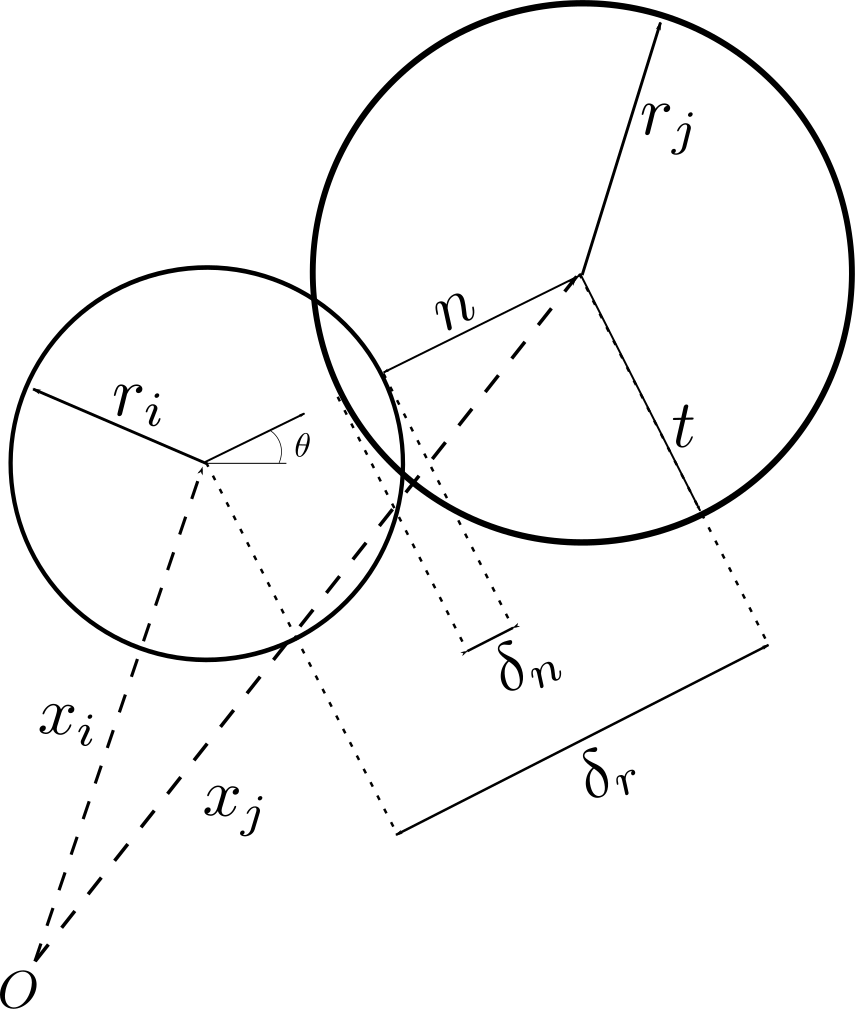
\includegraphics{DEM}
	\caption[Calculation of normal force]{Grains \textit{i} and \textit{j} in 
	contact, and the 
	separation $\delta_{n}$ is used to calculate the normal force} 
	\label{fig:DEM}
\end{figure}
where \textbf{n} and \textbf{t} are unit vectors, pointing in the normal and 
the tangential 
directions. The procedure adopted to calculate the normal and tangential forces 
are discussed.

%****************************************** %
\subsubsection*{Normal force}
When granular particles collide, part of the kinetic energy is dissipated as 
heat and the other 
part causes deformation of the particle. These deformations generate 
interaction forces. The 
grains 
are considered to be rigid while their contact is assumed to be soft. Thus, the 
grains do not 
change their shape, instead they overlap. The shapes of the particles are 
conserved on an average, 
after many collisions. The overlap at the contact is limited to very small 
deformations, which are 
achieved by defining a repulsive normal force that opposes the overlap. The 
mutual compression 
($\delta_{n}$) of the particles \textit{i} and \textit{j} is defined as:
\begin{align}
 \delta_{n}=\left|x_{\mathbf{i}}-x_{\mathit{j}}\right|-r_{i}-r_{j}
\label{eq:delta}
\end{align}
where $x_{\mathit{i}}$ and $x_{\mathit{j}}$ are the centres of the grains and  
$r_{\mathit{i}}$ 
and 
$r_{\mathit{j}}$ are their radii (see Figure \ref{fig:DEM}). When 
$\delta_{n}>0$, the two grains 
are not in contact, and there is no interaction. When $\delta_{n}<0$, the two 
grains overlap, and 
there 
is a repulsive normal force that pushes the two grains apart. The simplest 
model is to consider 
the 
contact as a linear spring with damping. The repulsive force depends linearly 
on $\delta_{n}$, and 
is controlled by the stiffness of the grain. The energy dissipation due to the 
interaction between 
grains is an intrinsic characteristic of the granular material and is 
incorporated by adding a 
damping force that opposes the relative velocity for the duration of the 
contact. The interaction 
force at the contact is idealized as a simple spring-dashpot system, with 
elastic and dissipative 
constants~\citep{Luding1994}. 
\begin{align}
 {{F}_{n}}=
\begin{cases}
0, & {{\delta}_{n}}>0 \\
-{{k}_{n}}{{\delta}_{n}}-{{\gamma}_{n}}\frac{d{{\delta}_{n}}}{dt}, & 
{{\delta}_{n}}<0 \\
\end{cases}
\end{align} 
The constant ${k}_{n}$ characterises the stiffness of the grain, and must be 
chosen sufficiently 
large so that the overlap between the grains remain small. Nevertheless, the 
solution has an 
undesirable property of generating an attractive force~\citep{Posch2005}. It 
arises just before 
the 
two particles separate. In this case, we have ${d{\delta_{n}}}$$/{dt} > 0$  
while $\delta_{n}$ 
approaches zero. To avoid the attractive force, the force is computed in two 
stages: a candidate 
force $\hat{F}_{n}$ is calculated, and verified whether it is non-negative:
\begin{align}
 {\hat{F}_{n}}=-{{k}_{n}}{{\delta}_{n}}-{{\gamma}_{n}}\frac{d{{\delta}_{n}}}{dt},
  \quad F_{n}=
\begin{cases}
0, & {\hat{F}} \le 0 \\
{\hat{F}}_{n}, & {\hat{F}} > 0 \\
\end{cases} \label{eq:nf}
\end{align} 
For pairwise collisions, the normal force $(F_{n})$ represented as 
${{k}_{n}}{{\delta}_{n}}+{{\gamma}_{n}}$ causes a decrease in the relative 
normal velocity of the 
particles by a factor $\epsilon$. This factor is the \textit{coefficient of 
restitution}, and is 
defined as $\epsilon\approx g'/g$, where \textit{g} is the absolute normal 
relative velocity 
before 
the collision and \textit{g'} corresponds to the post-collision value. The 
relative velocity, 
${d{\delta_{n}}}$$/{dt} > 0$, can be obtained by 
differentiating~\cref{eq:delta}. Thus we obtain:
\begin{equation}
\label{eq:vn}
\frac{d{\delta_{n}}}{dt}=(\mathbf{v}_{\mathit{i}}-\mathbf{v}_{\mathit{i}}).{\mathbf{n}}
\end{equation}
where $\mathbf{v}_{\mathit{i}}=dx_{\mathit{i}}/dt$ is the velocity of grain 
\textit{i} and 
$\mathbf{v}_{\mathit{j}}=dx_{\mathit{i}}/dt$ is the velocity of grain 
\textit{j}. The numerical 
integration of~\cref{eq:vn} yields the separation $\delta_{n}$ and permits us 
to generalise the 
model and treat the tangential forces as well, as explained in the next 
section. By integrating 
Newton's equation of motion it is found that the linear force corresponds to 
the co-efficient of 
restitution, which is defined as:
\begin{align}
\epsilon=exp(-\frac{\pi\gamma_{n}}{2m^{eff}}/\sqrt{\frac{Y}{m^{eff}}-{\frac{\gamma^{n}}{2m^{eff}}}^{2}})
\end{align}
% 
%%*************************************************************************************************************************************************
% %

\subsubsection*{Tangential force}
Granular particles are not perfect spheres, but have a complicated surface 
texture, therefore at 
oblique collisions, besides the normal force there is a tangential force too. 
Even perfectly 
smooth 
spheres exert a tangential force due to their bulk viscosity~\citep{Posch2005}. 
To build a heap of 
spheres on a flat surface, the particles as well as the surface has to be 
sufficiently rough, 
indicating the dependence of the tangential force on the surface properties of 
the granular 
materials. For realistic simulation of granular materials, it is important to 
consider the 
tangential force in Discrete Element Method. The tangential force is considered 
in a similar 
fashion as the normal force, arising from a spring stretched by the relative 
motion of the grain. 
Tangential forces are modelled by considering the relevant relative tangential 
velocity of the 
particle surfaces at the point of contact. The point of contact is an 
approximation, as the 
description of the normal force assumes a compression $\delta_{n}$, which 
implies a contact 
surface 
in 3-D or a contact line in 2-D. Assuming a tangential spring of length 
$\delta_{t}$ exerts an 
opposing force to the relative tangential displacements (ignoring the effect of 
relative rolling 
between the particles), the tangential force can be postulated similar to the 
normal force 
(~\cref{eq:vn}) as:
\begin{equation}
\label{eq:vt}
\frac{d{\delta_{t}}}{dt}=(\mathbf{v}_{\mathit{i}}-\mathbf{v}_{\mathit{i}}).{\mathbf{t}}
\end{equation}
This equation must also be numerically integrated, just like~\cref{eq:fma}. The 
grains are in 
contact when $\delta_{t}<0$, and when $\delta_{t}=0$, the grains no longer 
exert a force on each 
other. With these assumptions, $\delta_{t}$ can be calculated similar to the 
normal force. The 
tangential force is assumed to be governed by Coulomb's friction law.
\begin{equation}
\left|F_{\mathit{t}}\right|\le\mu F_{\mathit{n}} \label{eq:fric}
\end{equation}
where $F_{\mathit{t}}$ is the tangential force and $\mu$ is the friction 
coefficient. It is 
therefore necessary to constrain the tangential force to remain less than or 
equal to $\mu F_{N}$. 
To impose the condition in~\cref{eq:fric}, two-stages similar to the normal 
force computation is 
adopted. The first step is to evaluate the candidate force, and is then 
accepted if it obeys the 
condition in~\cref{eq:fric}.
\begin{align}
 {\hat{F}_{t}}=-{{k}_{t}}{{\delta}_{t}}-{{\gamma}_{t}}\frac{d{{\delta}_{t}}}{dt},
  \quad F_{t}=
\begin{cases}
sgn(F_{t}), & {\left|\hat{F}\right|} \ge \mu F_{n} \\
{\hat{F}}_{t}, & {\left|\hat{F}\right|} < \mu F_{n} 0 \\
\end{cases}
\label{eq:tf}
\end{align} 
where $k_{t}$ is the stiffness of the tangential spring and $\gamma_{t}$ is the 
damping constant. 
If $|F_{t}|=\mu F_{n}$, the contact is sliding, otherwise, it is non-sliding. 
It can noted that 
the 
normal force (~\cref{eq:nf}) and the tangential force (~\cref{eq:tf}) are 
handled in the same 
way in Discrete Element Method. When the grains slide against each other, they 
do not retain any 
memory 
of their initial position, and hence do not return to its original position. In 
order to model 
this 
behaviour, a limiting value of $\delta_{t}$ is imposed. When the contact slides 
$\delta_{t}=\pm\mu 
F_{n}/k_{t}$ is imposed.

In addition to sliding, the grains can roll relative to one another about their 
centre of mass due 
to the tangential force acting at their contact surface. In this case, 
$d\delta_{t}/dt=0$. It is 
important to assume that the grains touch at a single point instead of 
overlapping, i.e. 
$\delta_{n}=0$. This point is located at 
${x}_{\mathit{i}}-r_{\mathit{i}}\mathbf{n}={x}_{\mathit{j}}+r_{\mathit{j}}\mathbf{n}$.
 If we 
consider that this point belongs to grain $\mathit{i}$, its velocity is 
${v}_{\mathit{i}}+r_{\mathit{i}}(\mbox{\boldmath${\omega}$}\times\mathbf{n})$. 
If it belongs to 
grain \textit{j}, its velocity is 
${v}_{\mathit{j}}+r_{\mathit{j}}(\mbox{\boldmath${\omega}$}\times\mathbf{n})$. 
The relative 
velocity is the difference between these two velocities. 
\begin{equation}
\frac{d\delta_{t}}{dt}=(\mathbf{v}_{\mathit{i}}-{\mathbf{v}}_{\mathit{j}})\cdot 
\mathbf{t} 
-(r_{\mathit{i}} \mbox{\boldmath${\omega}$}_{\mathit{i}}
+r_{\mathit{j}}\mbox{\boldmath${\omega}$}_{\mathit{j}})\times\mathbf{n} 
\label{eq:rf}
\end{equation}
It should be noted that the~\cref{eq:rf} is only an approximation, as the 
grains in Molecular 
Dynamics do not touch at points, but overlap. It is therefore an approximation 
that produces an 
error of order $\mathbf{\mathit{O}}(\delta_{n}/r)$~\citep{Radjai2011}. It is 
assumed that the 
contact forces are exerted at the point of contact. It implies that the 
tangential force is 
accompanied by torque acting on two grains. If the overlap is zero, these 
torques are:
\begin{align}
\tau_{\mathit{ij}}=-(a_{\mathit{i}}\mathbf{n})\times(F_{t}\mathbf{t}), & 
\tau_{\mathit{ji}}=-(a_{\mathit{j}}\mathbf{n})\times(F_{t}\mathbf{t}),
\label{eq:av}
\end{align}
The torques modify the angular velocities of the grains. It is therefore 
necessary to incorporate 
the equation for the angular coordinates of the grains in~\cref{eq:fma}:
\begin{equation}
\mathit{I}_{j}\frac{d\omega_{i}}{dt}=\sum\limits_{j\ne i}{\tau_{ij}}
\end{equation}
where $\mathit{I}_{j}$ is the moment of inertia of grain j. The~\cref{eq:av} is 
only valid when 
$\delta_{n}=0$. The torque is a vector product of the force and its lever arm. 
It is assumed that 
the lever arms have lengths equal to $r_{\mathit{i}}$ and $r_{\mathit{j}}$, 
which is true only 
when 
the grains do not overlap, hence in this case they produce an error of order 
$\mathbf{\mathit{O}}(\delta_{n}/r)$. It is nevertheless desirable to damp this 
type of 
motion~\citep{Radjai2011}. 
The interaction between two solid bodies is much more complex than that is 
described by the simple 
linear model. Nevertheless, the linear force law has several advantages. It is 
simple to 
implement, 
and its harmonic behaviour is well understood, which makes it easier to 
interpret the results. The 
most common non-linear interaction law is the Hertz law~\citep{Hertz1882}. In 
certain situations, 
such as a quasi-static packing, a non-linear law can have significant influence 
on the acoustic 
properties~\citep{Tou2004}, and on the global stiffness~\citep{Agn2007}. 
However, in case of rapid 
granular flows, the interaction force between the particles has almost no 
effect on the 
phenomenon, 
and a linear law can be used to describe this kind of 
behaviour~\citep{Radjai2011}. 
% 
%%%***********************************************************************************************************************************************
% % %
%
\subsection{Numerical algorithm and integration scheme}
The efficiency of a Discrete Element Method program is mainly determined by 
its efficiency to compute the interaction forces between particles. If we 
consider a model system with pairwise interactions, we have to consider the 
contribution of the force on particle \textit{i} due to all its 
neighbours. If we consider only the interaction between a particle and the 
nearest image of another particle, then for a system of \textit{N} particles, 
we must evaluate $N \times (N-1)/2$ pair distances. Consider a system of 1000 
particles, at every time step all possible pairs of particles have to be 
considered to compute the interaction forces, hence, 
$\mathit{N}(\mathit{N}-1)/2 \approx 500,000$ 
force computations are required. For short-range particle interactions, the 
majority of these force evaluations is unnecessary as the corresponding 
particles are located far apart and do not necessarily touch each other. For a 
dense system of equally sized particles, the particles can have 
contacts with not more than 6 particles, this reduces the number of force 
computation required to $3\mathit{N} \approx 3000$. In the preliminary force 
computation scheme, at least 166 times more pair interactions are considered 
than necessary. Therefore, the numerical methods employed in the 
Discrete Element Method program should try to minimize the computation of 
interaction forces~\citep{Posch2005}. There are three different methods for the 
efficient computation of the forces, the \textit{Verlet} algorithm, the 
\textit{link-cell} algorithm, and a \textit{lattice} algorithm. The 
\textit{Verlet} algorithm described in~\citet{Grubmuller1991} 
is implemented in the 
present study.
\clearpage
\subsubsection{Verlet list algorithm}
The Verlet list algorithm assumes a cut-off value, so that only neighbouring 
particles that contribute to the energy of a particle \textit{i} are 
considered. It is advantageous to exclude the particles that do not interact in 
the memory expensive energy computation.~\citet{Verlet1967} 
developed a book-keeping technique, commonly referred to as the Verlet list or 
neighbour list, which is illustrated in~\ref{fig:Verletb}. In this method a 
second cut-off radius $r_{\mathit{v}}>r_{c}$ is introduced, and before we 
calculate the interactions, a list is made (the Verlet list) of all particles 
within a radius $r_{\mathit{v}}$ of the particle \textit{i}. In the 
subsequent calculations of the interactions, only those particles in this list 
will be considered. The idea of the Verlet algorithm is based on a simple 
property of particle dynamics: neighbourhood relation between particles can 
only change slowly, i.e. two particles which are close to each other 
at a given time step will remain as neighbours, at least in the following few 
time steps. During initialization the neighbourhood relations between the 
particles, i.e. the distance of all close 
pairs of particles are computed. Two particles are considered as neighbours if 
the distance of 
their surface is smaller than a predefined distance \textit{Verlet distance}:
\begin{figure}[htbp]	
\centering
\includegraphics[scale=0.75]{Verletb}
\caption[Verlet list]{The Verlet list: a particle \textit{i} interacts with 
those particles with 
the cut-off radius $r_{c}$, the Verlet list contains all the particles within 
a sphere with radius 
$r_{\mathit{v}>r_{c}}$}
\label{fig:Verletb}
\end{figure}
\begin{equation}
(\left|\overrightarrow{r_{\mathit{i}}}-\overrightarrow{r_{\mathit{j}}}\right|-\mathit{R}_{\mathit{i}}-\mathit{R}_{\mathit{j}})<\mbox{\textit{Verlet
 distance}}
\end{equation}

For each particle there is a \textit{Verlet list} in which the close 
neighbours are saved. To 
initialise the Verlet lists efficiently, a grid that covers the simulation 
area is defined. Its 
mesh size is larger than the largest particle. For construction of the lists 
only pairs whose 
particles reside in the same or adjacent grids are considered. This procedure 
guarantees the 
detection of all close pairs of particles~\citep{Posch2005}. Redundancy in 
Verlet lists, i.e. if 
particle \textit{i} is a neighbour of \textit{j}, then particle \textit{j} is 
a neighbour of 
\textit{i}, are avoided by imposing a restriction on the list of particle 
\textit{i} contains, 
such 
that it contains only neighbours with index $\mathit{j}<\mathit{i}$. For the 
computation of 
interaction forces, the Verlet list of particle \textit{i} is scanned and only 
pairs which are 
recorded in one of the Verlet lists are considered. Hence, the Verlet list of 
each particle 
\textit{i} is scanned and the interaction force of \textit{i} with each entry 
\textit{j} in its 
list is computed. Initially to build the Verlet list, the particles are sorted 
into a grid of mesh 
size $\mathit{dx}\times\mathit{dy}$. For each grid there is a list of 
particles residing in the 
cell. During the simulation, the neighbourhood relation among the particles 
change, therefore, the 
Verlet lists have to be updated. The decision to update a Verlet list depends 
on how far the 
particles have travelled since the time when the present list was built. The 
Verlet list of a 
particle \textit{i} must contain at any time all neighbours \textit{j} with 
$\mathit{j}<\mathit{i}$. This assures that two particles \textit{i} and 
\textit{j} never touch and 
are not considered as neighbours, i.e. \textit{j} is not in the list of 
\textit{i} and \textit{i} 
is not in the list of \textit{j}. Hence,
%
\begin{equation}
\left|\overrightarrow{r_{\mathit{i}}}-\overrightarrow{r_{\mathit{j}}}\right|-\mathit{R}_{\mathit{i}}-\mathit{R}_{\mathit{j}}>0
\end{equation}
%
The above condition is required for all pairs $(\mathit{i},\mathit{j})$ of 
particles which are 
\textit{not} known as neighbours. This condition is a criterion to update the 
Verlet 
lists~\citep{Posch2005}. Assume at the instant when the Verlet lists are 
constructed, the surfaces 
of the particles have the distance $\left| \overrightarrow{r_{\mathit{i}}} - 
\overrightarrow{r_{\mathit{i}}}\right| - 
\mathit{R}_{\mathit{i}}-\mathit{R}_{\mathit{j}} > 
\mbox{Verlet distance}
$, i.e. they are not classified as neighbours. If the 
Verlet lists are 
updated before one of these particles has travelled the distance 
$\mathit{verlet distance}/2$ 
since 
the lists were constructed, they can never collide without being recognized as 
neighbours first. 
This is explained in~\cref{fig:Verlet}. The impact of optimisation of the 
Verlet list 
algorithm has negligible effect on the computation time, as the algorithm is 
quite efficient 
already and only consumes a few percent of the total computation time in 
construction of the 
Verlet 
lists. The implementation of the Verlet list algorithm in force computation 
drastically reduces 
the 
computation time in comparison to the linear algorithm. The performance of the 
Verlet list 
algorithm is controlled by two crucial parameters: the number of cells 
$\mathit{N}_{\mathit{c}}$, 
for the construction of the Verlet lists and the Verlet distance 
$r_{\mathit{v}}$~\citep{Posch2005}.

\begin{figure}[htbp]
\centering
\includegraphics{Verlet}
\caption[Checking the validity of Verlet list]{Checking the validity of Verlet 
lists. 
\textit{Left}: the particles \textit{i} and \textit{j} are not recognized as 
neighbours since the 
distance of their surface is larger than the Verlet distance. The radius of 
the dashed circle is 
$\mathit{R}_{\mathit{i}}+\mathit{R}_{\mathit{max}}+\mbox{\textit{Verlet 
distance}}$. 
\textit{Right:} in the most unfortunate case the particles approach each other 
directly, 
travelling 
at the same velocity. As soon as one of the particles has travelled the 
distance $\mbox{\textit{Verlet distance}}/2$ (\textit{arrows}), the Verlet 
lists have 
to be rebuilt. The 
particles \textit{i} and \textit{j} are now recognized as neighbours. Figure 
redrawn after~\citet{Posch2005}.}
\label{fig:Verlet}
\end{figure}

\subsubsection{Leap frog or Verlet integration algorithm}
Discrete Element Method involves numerically solving Newton's equation of 
motion~\cref{eq:fma}, 
which 
is an ordinary differential equation. Choosing an integration algorithm is 
important, as the 
forces 
are not always differentiable in time, and the temporary derivative of the 
force is discontinuous 
when the contact splits. It is also very essential to numerically 
integrate~\cref{eq:rf} with 
the same precision as~\cref{eq:fma}. At first, computational speed seems 
important. It is 
usually not very relevant because the fraction of time spent on integrating 
the equation of 
motions 
(as opposed to computing the interactions) is small. Accuracy for large time 
steps is more 
important, because the larger the time step that we can use, the fewer 
evaluation of the forces 
are 
needed per unit of simulation time. Hence, this would suggest that it is 
advantageous to use a 
sophisticated algorithm that allows use of larger time step. Algorithms that 
allow the use of 
large 
time steps, achieve this by storing information on increasingly higher-order 
derivatives of the 
particle coordinates. Consequently, they tend to require more memory storage. 
However, the most 
important aspect to consider is the energy conservation. It is important to 
distinguish between 
two 
kinds of energy conservation: the short time and long time. The sophisticated 
higher-order 
algorithms tend to have very good energy conservation at short times. However, 
they often have 
undesirable feature that results in drifting of the overall energy for longer 
times. In contrast, 
the Verlet style algorithms tend to have only moderate short term energy 
conservation, but little 
long-term drift~\citep{Daan1996}. In this case, such algorithms are not 
useful. They are more 
complicated to program, and do not yield a more precise 
solution~\citep{Sean2011}. It might seem 
important to have an algorithm that accurately predicts the trajectories of 
all particles for both 
short and long durations, however no such algorithm exists. In certain cases, 
two trajectories 
that 
are initially very close may diverge exponentially as time progresses. Any 
integration error, 
however small it may be, would always diverge the predicted trajectory 
exponentially from the true 
trajectory. This phenomenon is called the Lyanpunov instability, and it is 
devastating to the 
whole 
idea of Discrete Element Method simulation, but we have good reasons to assume 
that even this 
problem 
need not be serious~\citep{Daan1996}. First of all, one should realize that 
the aim of the 
Discrete Element Method simulation is not to predict precisely what will 
happen to a system, but 
to 
predict the average behaviour of the system that was prepared in an initial 
state about which we 
know something (initial position, velocity and energy), but not everything. 
Hence, Molecular 
Dynamics technique differs from other methods, which are used to predict the 
trajectories. 
However, 
considerable numerical evidence suggest that the shadow orbits exists, which 
is a true trajectory 
of a multi-body system that closely follows the numerical trajectory for a 
time that is longer in 
comparison with the time that is required for the Lyapunov instability to 
develop~\citep{Daan1996}.

Newton's equations of motion are time reversible, and so should be the 
integration algorithm. The 
``leapfrog'' algorithm or the Verlet integration algorithm is a numerical 
scheme used to integrate 
the Newton's equation of motion to calculate the trajectories of particles and 
was implemented in 
Discrete Element Method simulation by~\citet{Verlet1967}. Verlet algorithm is 
fast and requires 
less 
storage memory, it is not particularly accurate for long time steps, and 
hence, we should expect 
to 
compute the forces on all particles rather frequently. Its short-term energy 
conservation is fair 
(in versions that use more accurate expression for velocity), but most 
importantly it exhibits 
little long-term energy drifts. This is related to the fact that the Verlet 
algorithm is time 
reversible and area preserving, however, it does not conserve the total energy 
of the system 
exactly~\citep{Daan1996}. Verlet algorithm is simply based on a truncated 
Taylor expansion of 
particle co-ordinates. 
\begin{equation}
t(t+\Delta t)=r{t} +\mathbf{v}(t) \Delta t + \frac{f(t)}{2\mathit{m}} \Delta 
t^{2}+ \dots
\end{equation}
If we truncate this expansion beyond the term $\Delta t^{2}$, we obtain the 
Euler's algorithm, 
which looks similar to the Verlet Algorithm, but it does not preserve energy 
and have significant 
energy drifts. The simplest among the Verlet schemes is the \textit{Leap frog 
algorithm}, which 
evaluates the velocities at half-integer time steps and uses these velocities 
to compute the new 
positions. The position of each grain is calculated at time $t=0, \Delta t, 
2\Delta t, $\dots$ ,$ 
where $\Delta t$ is the time step. On the other hand, their velocities are 
calculated at 
intermediate times, that is, at $t=\Delta t/2, 3 \Delta t/2, \dots,$. Let the 
position of a grain 
at time $t=k\Delta t$ be written as $x_{\mathit{k}}$, and its velocity at time 
$t=\Delta t (k + 
1/2)$ be written $\mathbf{v}_{\mathit{k + 1/2}}$, and its acceleration at $t=k 
\Delta t$ be 
$\mathbf{a}_{\mathit{k}}$. Then the following equation is used to advance 
systematically:
%
\begin{align}\label{eq:verlet}
\mathbf{v}_{\mathit{k}+1/2}=\mathbf{v}_{\mathit{k}-1/2}+\mathbf{a}_{\mathit{k}}
 \Delta t, \qquad & 
x_{\mathit{k}+1}=x_{\mathit{k}}+\mathbf{v}_{\mathit{k}+1/2} \Delta t
\end{align}
%
This algorithm determines the new grain position with an error of order 
$\mathit{O}( \Delta 
t^{4})$. But~\cref{eq:verlet} hides a difficulty in the application of this 
algorithm to 
granular materials~\citep{Radjai2011}. The problem is that the acceleration 
must be calculated at 
time $t=k\Delta t$. But the velocities are known at $t=(k - 1/2) \Delta t$, 
and not at $t=k \Delta 
t$. One way to get around this problem is to write:
%
\begin{equation} 
\mathbf{v}_{\mathit{k}}={\mathbf{v}_{\mathit{k}-1/2}+{\mathbf{a}_{\mathit{k}-1}\Delta
 t/2}}
\label{eq:ver}
\end{equation}
%
The equation uses the acceleration of the preceding time step to estimate the 
velocity. This 
approximation does not diminish the order of the algorithm.~\cref{eq:ver} 
estimates 
$\mathbf{v}_{k}$ with an error of order $\mathbf{O}(\Delta t^{2})$, which 
produces an error of the 
same order in the calculation of the force in~\cref{eq:verlet}. But this 
causes only an error of 
order $\mathbf{O}(\Delta t^{3})$ in the velocity and an error of order 
$\mathbf{O}(\Delta t^{4})$ 
in the position. However, this problem does not exist in energy conservation 
systems, because the 
computed forces do not depend on the velocities of the grains. The heaviest 
computational task is 
the evaluation of forces and not the integration of equations. The Verlet 
integration scheme is 
summarized in~\cref{eq:vers} and~\cref{fig:verlet}. To calculate the forces 
and 
acceleration, it requires the positions and velocities at time t:
%
\begin{align}
& \mathbf{v}(t+\Delta t/2)=\mathbf{v}(t-\Delta t/2) + \mathbf{a}(t) \Delta t 
\nonumber \\
& x(t+\Delta t)=x(t)+\mathbf{v}(t+\Delta /2) \Delta t \nonumber \\
& \mathbf{v}(t)=\mathbf{v}(t-\Delta t /2)+\mathbf{a}(t- \Delta t) \Delta t /2
\label{eq:vers}
\end{align}

\begin{figure}[htbp]
\centering
\includegraphics{Leap}
\caption{Verlet integration scheme}
\label{fig:verlet}
\end{figure}
The analysis of the Discrete Element Method formulation reveals that the linear 
force law gives 
the 
model a harmonic character, showing that it is very closely related to simple 
models widely used 
in 
physics and mechanics. The shortest time scales often arise from the 
oscillations of one or two 
grains. The integration algorithm must resolve these movements with sufficient 
precision. Thus, 
the 
time steps used must be smaller than these time scales, the most rapid 
frequency is usually 
${\omega}_{\mathit{N}}$, the characteristic oscillation frequency of very short 
waves. This 
frequency is proportional to $\omega _{o}$, which is easier to estimate. 
Therefore, it is 
essential 
to choose a time step $\Delta t \approx \epsilon / \omega_{0}$, where 
$\epsilon$ is a constant 
that 
depends on the integration algorithm. Values such as $\epsilon \approx 0.01$ 
are often a 
reasonable 
choice~\citep{Sean2011}. In the case of rapid granular flows, the time step 
must be small enough 
so 
that the fastest grains move only by a small fraction of their size during one 
time step. The 
grains must be stiff enough so that violent collisions do not lead to large 
overlaps between 
particles. 
%%*************************************************************************************************************************************************************************
%% %
\subsection{Boundary conditions}
In many cases, the dynamic and static properties of a granular system are 
substantially affected 
by 
the interaction of the granular material with the system boundaries, i.e. by 
the properties of the 
container or the surface on which the material is present. The effect of 
boundary conditions on 
the 
response of the granular assembly can be noticed in the convective motion of 
granular material in 
vibrating containers, the formation of density waves in pipes, the motion of 
granular material on 
conveyors, and the clogging of hoppers. In these and many other cases, careful 
definition of the 
interaction between the granular material and the contact surface is essential. 
Of particular 
importance is the realistic modelling of the wall surface roughness. 
Unfortunately the mechanical 
interaction of a granular materials with a rough wall is poorly 
understood~\citep{Posch2005}. A 
simple way to define the wall property is to build up the wall from particles, 
which obey the same 
rules of interaction as the particles of granular material. By varying the size 
and position of 
the 
wall particles, system boundaries of adjustable roughness can be described. 
However, the surface 
roughness that characterizes the frictional properties of the wall has to be 
arrived iteratively, 
and may not represent the real conditions. In the present case, a solid wall 
with corresponding 
stiffness, damping and frictional characteristics is introduced to model the 
interaction between 
particles and the wall. The interaction force is computed in a similar fashion 
to that of a pair 
of 
particles in contact and is divided into the normal and tangential components. 
The compression of 
the particle upon collision with the wall is calculated along the normal 
direction to the wall and 
the particle contact.   

\subsubsection{Periodic boundary} \label{periodic}
The effect of a wall on the response of particles is very critical, especially 
in numerical 
simulation where the number of particles is relatively fewer in comparison to 
the experiments. The 
undesired effect of a wall can be eliminated using periodic boundary 
conditions, i.e. a periodic 
extension of the simulation area in one or more dimensions. Any particle 
leaving the system at one 
side is reintroduced at the opposite side, and correspondingly the interaction 
forces between 
particles at opposite sides of the simulation area are taken into account. In 
this framework, the 
simulation domain becomes a unit area containing particles with periodic copies 
paving the whole 
system. The periodic boundary conditions extend the system boundaries to 
infinity, so that the 
simulation cell simply plays the role of a coordinate system to locate particle 
positions~\ref{fig:periodic}. 

The external stresses or displacements are applied on the simulation box by 
constraining the 
degrees of freedom of the wall, which are alternatively kept free or fixed 
depending on whether a 
stress or a displacement is monitored in a system. With periodic boundary 
conditions, this role is 
played by the collective degrees of freedom carried by the coordinate system, 
whose basis vectors 
become dynamic variables, and their conjugate stresses are expressed as a state 
function of the 
granular configuration~\citep{Par1980}. In the case of granular systems, there 
is dissipation of 
energy during particle interactions. The kinematics, equation of dynamics, and 
the time-stepping 
schemes for Discrete Element Method are discussed in detail 
in~\citet{Voiv2011}. The periodicity 
in 
position implemented in the present study is discussed below. 
\begin{figure}[htbp]
\centering
\includegraphics[scale=0.65]{periodic}
\caption[A 2D simulation cell $\omega$ with its basis vectors in an absolute 
frame]{A 2D 
simulation 
cell $\omega$ with its basis vectors in an absolute frame. A particle located 
at the right 
boundary 
interacts with the image of another particle located at the left boundary.}
\label{fig:periodic}
\end{figure}

Let us consider a collection of $N_{p}$ particles with their centres contained 
in a cell of volume 
V . The cell can have any shape allowing for a periodic tessellation of space. 
The simplest shape 
is a parallelepiped i.e. parallelogram in 2D. The cell and its replicas define 
a regular lattice 
characterized by its basis vectors 
$(\overrightarrow{\mathbf{a}_{1}},\overrightarrow{\mathbf{a}_{2}})$. In the 
case of a 
parallelogram, the basis vectors may simply be the two sides of the 
parallelogram; 
~\cref{fig:periodic}. The origin \textit{O} of the simulation cell is a vertex 
of the cell of 
coordinates (0, 0) and its replicas are defined by two indices $(i_{1}, i_{2})$ 
corresponding to a 
translation of the origin by the vector 
$i_{1}\overrightarrow{\mathbf{a}_{1}}+i_{1}\overrightarrow{\mathbf{a}_{2}}$. 
Then, the coordinates 
$\overrightarrow{r}(\mathit{i})$ of the image $\mathit{i}^{\prime}$ of a 
particle $\mathit{i} \in 
\Omega$ of coordinates  $\overrightarrow{r}(\mathit{i}^{\prime})$ are given by:
\begin{align}
\overrightarrow{r}(i^{\prime})=\overrightarrow{r}(i)+\sum\limits_{k=1}^{2}{\mathit{i}_{\mathit{k}}\overrightarrow{\mathbf{\mathit{a}}}_{\mathit{k}}}
\end{align}
The particles belonging to the cell $\Omega$, characterized by $\mathit{i}_{1} 
= \mathit{i}_{2} = 
0$, can interact with the particles of the same cell but also with image 
particles in the 
neighbouring cells characterized by $\mathit{i}_{k}\in {1, 1}$. There are  
$3^{D} - 1$ cells 
surrounding the simulation cell and they are involved in the search of contact 
partners for each 
particle. The distance between two particles \textit{i} and \textit{j} $\in 
\Omega$ is the 
shortest 
distance separating \textit{i} from \textit{j} or from one of its images 
$\mathit{j}^{\prime}$. As 
the system evolves in time, a particle \textit{i} may leave but one of its 
images 
$\mathit{i}^{\prime}$ enters at the same moment. In order to keep all original 
particles in the 
cell, the status ``original'' should be reserved to the particles whose centres 
belongs to 
$\Omega$. Hence, whenever a particle \textit{i} leaves the simulation cell, it 
becomes an image of 
$\mathit{i}^{\prime}$, which then becomes the original. This means that a 
particle crossing a 
border of the simulation cell, returns to the cell by crossing another border.
%%***********************************************************************************************************************************************
%% %
\subsection{Particle Assembling Methods}
In order to simulate a granular assembly, it is essential to assign an initial 
position and 
velocity to all the particles in the system. Particle positions should be 
chosen to be compatible 
to the structure (granular fabric) we are trying to simulate. In any event, the 
particles should 
not be positioned such that there is an appreciable overlap between particles. 
In order to achieve 
the initial position of the particles, various particle-assembling methods can 
be adopted. The 
particle assembling methods can be classified into two broad categories: 
dynamic methods and 
geometrical approaches. The dynamic approach involves packing of grains using 
laws of mechanics 
and 
contacts, while in the geometrical method the particles are packed considering 
their geometry, 
i.e. 
grain size, shape and its position. In general, the packing of particles can be 
categorized into 
two types: crystal/lattice packing, like hexagonal or square pattern of 
mono-disperse particles, 
and random packing with varying density employing mono-disperse or 
poly-disperse grains. The 
crystalline packing arrangements, such as hexagon and square lattices, are 
easier to generate, 
however they have non-trivial effects on the response of the granular 
system~\citep{Staron2005}. 
Hexagonal packing is the densest possible arrangement for mono-dispersed 
spherical grains. In 2D, 
the packing of mono-dispersed circles on a hexagonal lattice yields a packing 
density of 
$\eta_{\mathit{h}}=\frac{1}{6}\pi\sqrt{3}\approx 0.9068$
%.~\cref{fig:sqhex} shows a typical hexagonal lattice arrangements of grains in 
%a 2D granular 
%column.
%\begin{figure}[htbp]
%\centering
%\includegraphics[scale=0.25]{Hexagon}
%\caption{Hexagonal lattice arrangement of grains}
%\label{fig:sqhex}
%\end{figure}

The rheology of a granular material is controlled by the geometry of the 
assembly, which includes 
the particle shape, size distribution, and their arrangement. This prevailing 
role of geometry 
sometimes permits to simplify the dynamics in favour of a better description of 
the geometry 
and/or 
higher numerical efficiency~\citep{Radjai2011}. For example, dense granular 
packing may be 
efficiently constructed by replacing the equations of dynamics by simple 
displacement rules 
satisfying the geometrical constraints. Purely geometrical procedures can be 
much simpler and 
numerically faster than dynamic or quasi-static methods. Contrary to dynamic 
simulation methods, 
the geometrical methods allow for quick assembling of a large number of 
particles. Such packing 
may 
then be used as the initial state for dynamic simulations. The issue of the 
assembling methods is 
to construct configurations of particles as close as possible to a state of 
mechanical equilibrium 
with built-in packing properties. This can be a target packing density for a 
given particle size 
distribution. In the same way, the average connectivity of the particles 
(coordination number) and 
the anisotropy of the contact network are basic geometrical properties. The 
coordination number 
represents the mechanical response of packing. The homogeneity of the particle 
assembly in terms 
of 
packing fraction and connectivity is another important property, which depends 
on the assembling 
rules. In the present study, the initial grain packing is obtained using 
ballistic deposition 
technique.

\subsubsection{Ballistic deposition}
Initially a random arrangement of particles which do not touch each other is 
generated 
(~\cref{fig:ini}). The radii of the particles are chosen from the interval of 
$(\mathit{R}_{\mathit{min}},\mathit{R}_{\mathit{max}})$ in such a way that the 
total mass of all 
particles from a certain size interval is the same for all sizes, thus ensuring 
that neither 
larger 
nor smaller particles dominate the system. This distribution can be obtained, 
if the radii are 
chosen according to the probability distribution:
\begin{align}
\mathit{p}(\mathit{R})=\frac{\mathit{R}_{\mathit{min}}\mathit{R}_{\mathit{max}}}{\mathit{R}_{\mathit{max}}
 - \mathit{R}_{\mathit{min}}} \frac{1}{\mathit{R}^{2}}
\end{align}
Random numbers according to the above distribution can be generated from 
equi-distributed random 
numbers $\mathit{z}\in [0,1]$ via the transformation
\begin{align}
\mathit{R}=\frac{\mathit{R}_{\mathit{min}}\mathit{R}_{\mathit{max}}}{\mathit{R}_{\mathit{max}}
 - 
z(\mathit{R}_{\mathit{max}} - \mathit{R}_{\mathit{min}})}
\end{align}
This transformation is applied to initialise the particle radii and the 
particles are arranged 
randomly on a regular lattice. The configuration of particles obtained after 
this step is 
presented 
in~\cref{fig:ini}.
%\begin{figure}[htbp]
%\centering
%\includegraphics[scale=0.23]{ini}
%\caption{Radom polydisperse particles arranged in a regular lattice, showing 
%the variation in the 
%particle size}
%\label{fig:ini}
%\end{figure}
In the second step, the particles arranged in a regular lattice are allowed to 
fall down and are 
packed using the \textit{random deposition with relaxation method}, a ballistic 
deposition 
technique. The geometrical methods help in this way to improve numerical 
efficiency in the 
preparation phase. For example, gravitational deposition of particles located 
initially on a 
regular grid can require hours of computation whereas a nearly similar result 
may be obtained by 
means of a geometrical method in only a few minutes. The drawback is that the 
resulting sample 
will 
not be in mechanical equilibrium and no information is available on the contact 
forces. 
Nevertheless, depending on the relaxation rule, the sample may still be 
sufficiently close to 
equilibrium to be considered as a good starting point for mechanical 
simulations. Hence, a 
combined 
approach of ballistic deposition and Discrete Element Method is adopted in the 
present study 
to generate mechanically stable samples. The random deposition and relaxation 
method, first 
proposed by~\citet{vold1959a,vold1959b} and developed by~\citet{jullien1992} 
and 
\citet{meakin1985}, is adopted in the present study. The general principle of 
this method is quite 
simple (see~\cref{fig:ballistic}); it consists of placing the particles 
consecutively on a 
substrate or a layer of already deposited particles. Each particle first 
touches the substrate or 
a 
deposited particle, then undergoes a relaxation process (single-particle 
restructuring) along the 
steepest descent (steepest-descent model) until a more stable position 
according to a stability 
criterion is reached. The construction of the packing proceeds layer by layer 
from the substrate, 
hence this deposition model is also known as bottom-to-top restructuring model. 
The first step is 
to release a particle from a random position above the substrate. Upon contact 
with the first 
deposited particle, the particle rolls following the steepest descent until a 
new contact is 
formed 
with a second particle. In 2D, two contacts are sufficient to balance a 
particle if its centre of 
gravity lies between the two contacts. This corresponds to a position of local 
stable equilibrium. 
If this criterion is not met, the particle continues to roll and the procedure 
is iterated until a 
local stable position is reached. The wall effects are eliminated by adopting 
periodic boundaries 
(Sec~\ref{periodic})in the horizontal direction (perpendicular to that of 
deposition). 
~\cref{fig:ballistic} shows a small sample prepared by this method (the grey 
particles are 
periodic images of the black ones). In this method, the order of deposited 
particles is generally 
random and independent of their sizes. The mechanically stable sample obtained 
from equilibrating 
the random deposited and relaxed sample is presented in~\cref{fig:sample} 
\begin{figure}[htbp]
\centering
\includegraphics[scale=0.1]{ballistic}
\caption{(a)\textit{Ballistic deposition}: first contact followed by steepest 
descent; (b) 
small-scale periodic sample~\citep{Radjai2011}}
\label{fig:ballistic}
\end{figure} 

%\begin{figure}[htbp]
%\centering
%\includegraphics[scale=0.23]{sample1}
%\caption[Mechanically stable sample prepared by ballistic deposition 
%technique]{Mechanically 
%stable 
%sample prepared by ballistic deposition technique and Molecular 
%Dynamics, showing the number of contacts per particle, the highlighted 
%portions are used as 
%representative elements in the statistical analysis}
%\label{fig:sample}
%\end{figure}

\subsubsection{Statistical analysis of prepared sample}
In order to ensure the homogeneity of the sample prepared using the above 
technique, a statistical 
analysis of the sample is performed. Various parameters such as particle size, 
coordination 
number, 
contact normal direction, contact normal force, etc., can be used in the 
statistical analysis to 
verify the homogeneity of the prepared sample. Of the various parameters 
available, the 
coordination number, i.e. the average number of contacts per particle is chosen 
to study the 
homogeneity of the sample, because of its simplicity and its physical 
significance in representing 
the density of the sample. With increase in the coordination number, the 
density of the granular 
assembly increases. The mechanically stable sample prepared by ballistic 
deposition technique 
presented in~\cref{fig:sample} is used for the statistical analysis. 
Representative elements 
of size 0.02 m $\times$ 0.01 m (highlighted segments in~\cref{fig:sample}) were 
considered. 
Each representative element has approximately 40 particles. A histogram is 
plotted showing the 
number of particles having a particular coordination number for all the 
representative elements 
(~\cref{fig:Hist}). A normal distribution of the number of particles and the 
coordination 
number can be observed from~\cref{fig:Hist}. Most particles are found to have 2 
or 3 contacts 
with its neighbours. The number of particles with higher coordination number, 
i.e. coordination 
number greater than 3, is found to increase as we go down the sample. This is 
attributed to the 
effect of gravity, which increases linearly as we go down. Representative 
elements at the top are 
found to have a shift in their peak towards lower coordination number, as they 
are less restrained 
in comparison to their counterparts at the bottom of the sample. Overall, the 
sample is found to 
be 
homogeneous, with representative elements having similar normal distribution of 
the coordination 
number. Thus, the prepared sample is a good representation of the actual 
granular assembly and the 
simulations based on these samples are found to be more realistic in comparison 
to 
crystalline/lattice packing of granular particles. 
%\begin{figure}[htbp]
%\centering
%\includegraphics[scale=0.6]{Hist}
%\caption[Statistical analysis of the sample prepared by ballistic deposition 
%technique]{Histogram 
%showing the variation in the number of particles with the coordination number 
%for 9 
%representative 
%elements from the sample in~\cref{fig:sample}}
%\label{fig:Hist}
%\end{figure} 

\subsection{Voronoi Tesselation}
\begin{figure}[tbhp]
\centering
\begin{subfigure}[b]{0.95\textwidth}
\centering
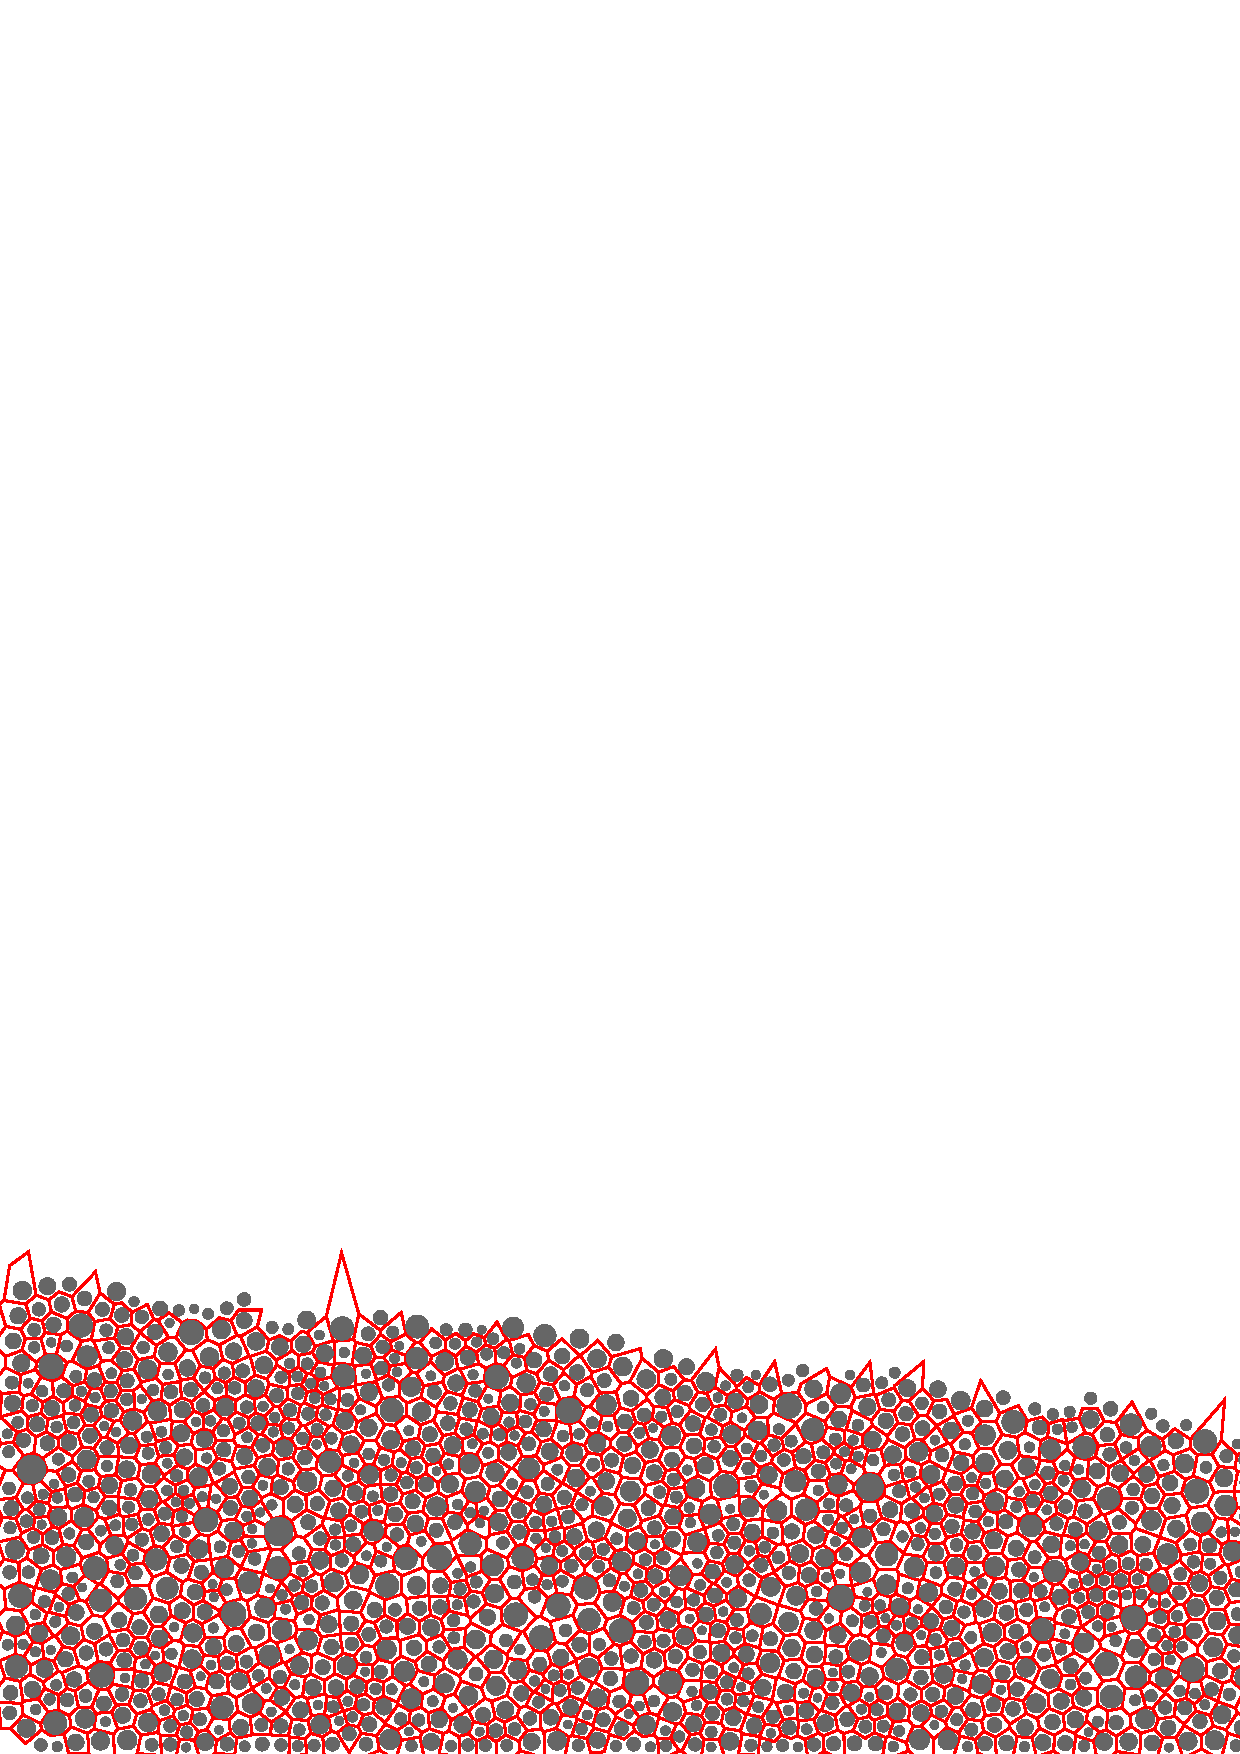
\includegraphics[width=\textwidth]{tesselation}
\caption{Voronoi Tesselation}
\label{fig:tesselation}
\end{subfigure}
\\
\begin{subfigure}[b]{0.95\textwidth}
\centering
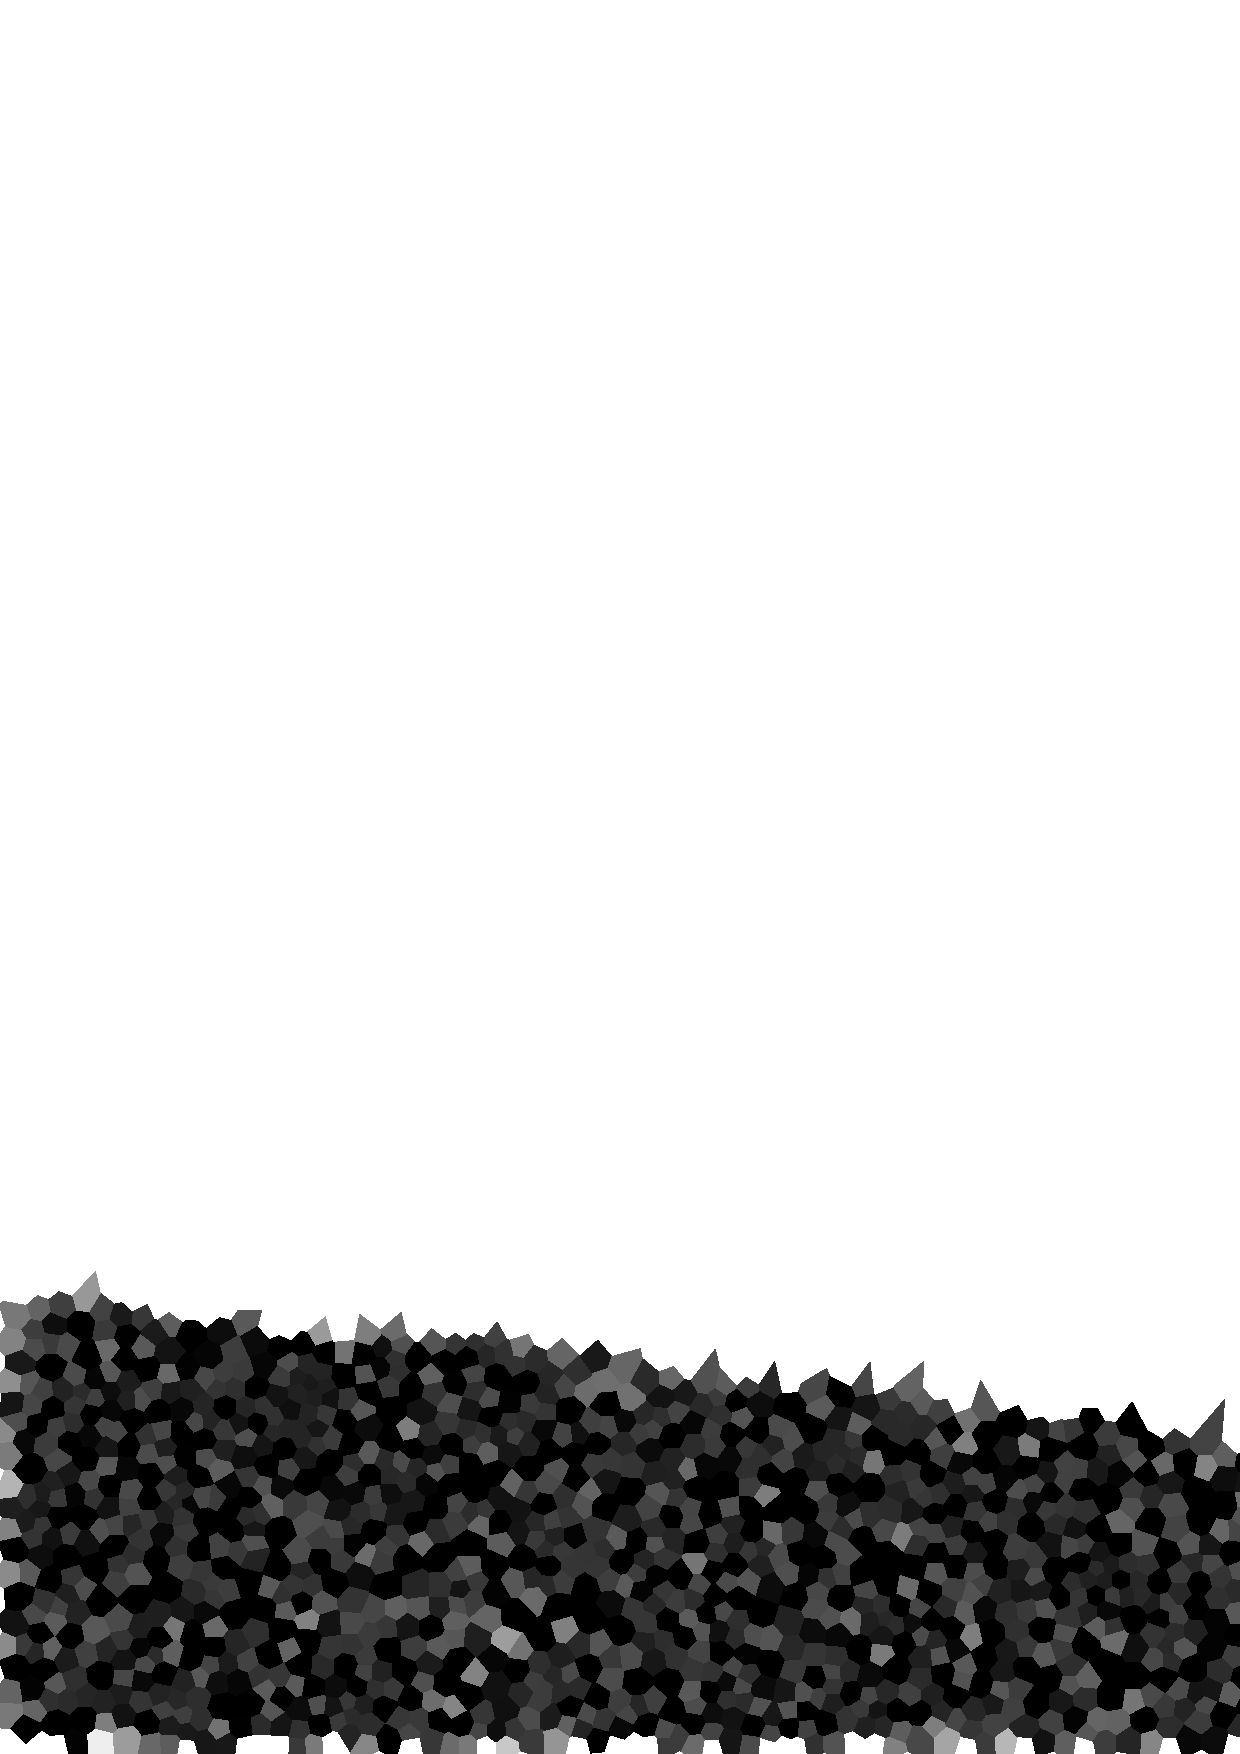
\includegraphics[width=\textwidth]{local_density}
\caption{Local packing density (dark - dense and light - loose)}
\label{fig:local_density}
\end{subfigure}
\caption{Voronoi tessellation to average bulk properties}
\label{fig:voro}
\end{figure}
